\documentclass[aspectratio=1610,10pt]{beamer} %Other possible values are: 169, 149, 54, 43 and 32.
  
\usepackage{amsmath,amsthm,amsfonts,amssymb,amscd, amsxtra, mathrsfs}
\usepackage{url}
\usepackage{bbm}
\usepackage{color}
\usepackage{xcolor}
\usepackage{lmodern}
\usepackage{graphicx,float}
\usepackage{pdfsync}
\usepackage{lineno}
\usepackage[labelfont=bf]{caption}
\usepackage{siunitx} %% Sistema Internacional de Unidades
\usepackage{multicol}

\usepackage{changepage}
\usepackage{ragged2e}
%\usepackage{biblatex}
%\usepackage{enumitem}
%\usepackage{microtype,todonotes}
\usepackage{lipsum}
\usepackage{booktabs}
\usepackage{tabularx}
\usepackage{colortbl}
\usepackage{xspace}
\usepackage{geometry}
\usepackage[scale=2]{ccicons}
%\usepackage{enumitem}
\usepackage{enumerate}
\usepackage{subfigure}
\usepackage{subfigmat}
\usepackage[T1]{fontenc} 
% \usepackage{caption}
% \usepackage{subcaption}
\usepackage{float}

%\usepackage{hyperref}


%\usepackage[compact,small]{titlesec} % Muda o tamanho e a fonte do título das seções
%\setlength{\parskip}{1.2ex} % tamanho do espaço entre uma linha e um parágrafo
%\setlength{\parindent}{0em} % tamanho do espaço no inicio de um parágrafo

% As viúvas e os órfãos são linhas no início ou no final de um parágrafo que ficam penduradas 
% no topo ou no final de uma página ou coluna, separadas do resto do parágrafo.
%\clubpenalty = 10000  % orfãos
%\widowpenalty = 10000.% viuvas

% Fontes alternativas
%\usepackage{kpfonts}

%  Define as cores a serem usadas
\definecolor{UFGblue}{rgb}{0.0039, 0.3529, 0.6431} 
\definecolor{UFGred}{HTML}{990000}
\definecolor{UFGorange}{rgb}{0.9216, 0.4863, 0.0784}
\definecolor{UFGgreen}{rgb}{0.0509, 0.4509, 0.1568}
\definecolor{UFGgray}{rgb}{0.3686, 0.5255, 0.6235} % UBC Gray (secondary)
\definecolor{ultramarine}{rgb}{0, 0.125, 0.376} 
\definecolor{UFGorange}{rgb}{0.9216, 0.4863, 0.0784}%{HTML}{EB811B}
\definecolor{UFGred}{HTML}{990000}

\newcommand{\red}[1]{\textcolor{UFGred}{#1}}
\newcommand{\blue}[1]{\textcolor{UFGblue}{#1}}
\newcommand{\green}[1]{\textcolor{UFGgreen}{#1}}
\newcommand{\gray}[1]{\textcolor{UFGgray}{#1}}


% definindo as margens do documento
%\geometry{a4paper,text={16.5cm,25.5cm},centering}

%preambulos separados
%\input{\string~/Projetos/ufg/preambles/geometry}
%\input{\string~/Projetos/ufg/preambles/newcomands}
%\input{\string~/Projetos/ufg/preambles/numerations}


% Colorinlistoftodos package: to insert colored comments so authors can collaborate on the content.
%\usepackage[colorinlistoftodos, textwidth=20mm, textsize=footnotesize]{todonotes}
%\newcommand{\aluno}[1]{\todo[author=\textbf{Aluno},color=green!30,caption={},inline]{#1}}
%\newcommand{\max}[1]{\todo[author=\textbf{Max},color=red!30,caption={},inline]{#1}}
\usepackage{xcolor}
\usepackage{graphicx}
\usepackage{ifthen}
\usepackage{xifthen}
\usepackage{amssymb,amsmath,amsthm}
\usepackage{pgf,pgfplots,pgfkeys}
\usepackage{tikz}
\usepackage{tkz-euclide}
\usepackage{siunitx} %% Sistema Internacional de Unidades
\usepackage{caption}


%\usepackage{tkz-fct}

%
%%! For older versions of package tkz-euclide
%%! you may need uncomment the following line:
%   \usetkzobj{all}
%%!

\usetikzlibrary
    {
      shapes.geometric,
      arrows,
      calc,
      intersections,
      arrows.meta,
      decorations.markings,
      positioning,
      math,
      angles,
      quotes,
      patterns,3d,
      backgrounds,
      fillbetween,
      automata,
      trees,
      external
    }


%%..
%%Usage: \gettikzxy{(P)}{\px}{\py}
\makeatletter
\newcommand{\gettikzxy}[3]{%
  \tikz@scan@one@point\pgfutil@firstofone#1\relax
  \edef#2{\the\pgf@x}%
  \edef#3{\the\pgf@y}%
  \tikzmath{#2=#2/28.3465;};
  \tikzmath{#3=#3/28.3465;};
}
\tikzstyle{bag} = [align=center]
\makeatother


\pgfplotsset{compat=1.18}

\usepgfplotslibrary{groupplots}


% to Bezier curves
\newcommand\DrawControl[3]{
  node[#2,circle,fill=#2,inner sep=2pt,label={above:$#1$},label={[black]below:{\footnotesize#3}}] at #1 {}
 }


\usepackage{refcheck} % coloca a referência no texto
\usepackage{biblatex}
\usepackage[english]{babel}

%------------------------------------ hyperrref
% \hypersetup{colorlinks,linkcolor={purple},citecolor={purple},urlcolor={purple}}  


\mode<presentation>
\usetheme{metropolis}
\setbeamercovered{transparent}

\newcommand{\themename}{\textbf{\textsc{metropolis}}\xspace}

\usefonttheme[onlymath]{serif}
\usefonttheme{structurebold} % fonte modo matematico


%  Define as cores a serem usadas
\definecolor{mLightBrown}{HTML}{990000} % alert block
\definecolor{mLightGreen}{HTML}{EB811B} % example text



% logo of my university
\titlegraphic{\vspace{4cm}\hfill
\includegraphics[height=2.3cm]{../figures/ufglogo.png}}


%Colocando um marca dagua
\setbeamertemplate{background}{
  \tikz[overlay,remember picture]
  \node[opacity=.05] at (11,-5.5) {
\includegraphics[width=10cm]{../figures/marcadagua.png}};
}


% - Define a cor da página
\setbeamercolor{background canvas}{bg=UFGblue!5}

% Define a cor da letra
\setbeamercolor{normal text}{fg=black}
%\setbeamercolor{example text}{fg=UFGgreen}
%\setbeamercolor{alerted text}{fg=UFGorange}


% Definindo as cores do palette
% Com cor no fundo do títulp
%\setbeamercolor{palette primary}{bg= UFGblue!30,fg=UFGblue!90!black}
%sem com no fundo do título
\setbeamercolor{palette primary}{bg= ,fg=UFGblue!90!black}
%\setbeamercolor{palette secondary}{bg=UFGblue,fg=white}
%\setbeamercolor{palette tertiary}{bg=UFGlue,fg=white}
%\setbeamercolor{palette quaternary}{bg=UFGblue,fg=white}l%


% tirando a cor dos cabeçalhos dos blocks
\setbeamercolor{block title}{bg= ,fg=UFGblue!90!black}
\setbeamercolor{block title example}{bg=}
\setbeamercolor{block title alerted}{bg=}


% Outras cores
% \setbeamercolor{structure}{fg=UFGblue} % itemize, enumerate, etc
% \setbeamercolor{section in toc}{fg=UFGblue} % TOC sections
% \setbeamercolor{title}{bg=UFGgrey}
% \setbeamercolor{item}{fg=green}
% \setbeamercolor{block body alerted}{bg=alerted text.fg!10}
% \setbeamercolor{block body}{bg=UFGblue!20}
% \setbeamercolor{block body example}{bg=UFGgreen!20}
%\setbeamercolor{block body alerted}{bg=UFGblue!10}
% \setbeamercolor{block title alerted}{bg=UFGred, fg=white}


% Transparencia dos blocks
%\addtobeamertemplate{block begin}{\pgfsetfillopacity{1}}{\pgfsetfillopacity{1}}
%\addtobeamertemplate{block alerted begin}{\pgfsetfillopacity{1}}{\pgfsetfillopacity{1}}
%\addtobeamertemplate{block example begin}{\pgfsetfillopacity{1}}{\pgfsetfillopacity{1}}


% % Override palette coloring with secondary
% \setbeamercolor{subsection in head/foot}{bg=UFGblue,fg=white}
% \setbeamercolor{section in head/foot}{bg=UFGgreen,fg=white}
% \setbeamertemplate{enumerate items}[default]
% \setbeamercolor{enumerate item}{fg=UFGblue}


% Desativando o cabeçalho
%\setbeamertemplate{headline}{}

% Colocando numero de paginas no slide
\setbeamertemplate{footline}{}

% Tela cheia
\hypersetup{pdfpagemode=FullScreen}

% justificando o texto nos blocks
\addtobeamertemplate{block begin}{}{\justifying}  %new code
\addtobeamertemplate{block example begin}{}{\justifying}  %new code
\addtobeamertemplate{block alerted begin}{}{\justifying}  %new code

% justificando o texto fora dos blocks
\apptocmd{\frame}{}{\justifying}{}

% Configurações da faixa nos frametitles
\makeatletter
\setlength{\metropolis@frametitle@padding}{1.3ex}%  <- largura da faixa
\setbeamertemplate{frametitle}{%
  \nointerlineskip%
  \begin{beamercolorbox}[%
      wd=\paperwidth,%
      sep=3pt,% 
      leftskip=\metropolis@frametitle@padding,%
      rightskip=\metropolis@frametitle@padding,%
    ]{frametitle}%
    \metropolis@frametitlestrut@start%
    \insertframetitle%
    \nolinebreak%
    \metropolis@frametitlestrut@end%
  \end{beamercolorbox}
}
\makeatother

\setbeamertemplate{itemize body end}{\vspace{2cm}}
\setbeamertemplate{itemize items}[default]

% Configuração dos frames
% \setbeamersize{
%     text margin left    = .06\paperwidth,
%     text margin right   = .03\paperwidth,
%     sidebar width left  = 0mm,
%     sidebar width right = 10mm,
%     description width   = 10mm,
%     mini frame size     = 10mm,
%     mini frame offset   = 10mm
% }

\makeatletter
\setlength\beamer@paperwidth{16.00cm}
\setlength\beamer@paperheight{10.00cm}
\geometry{%
  papersize={\beamer@paperwidth,\beamer@paperheight},
  hmargin=1cm,% 
  vmargin=0cm,%
  head=0.5cm,% might be changed later 
  headsep=0pt,%
  foot=1.5cm% might be changed later 
}
\makeatother

\counterwithout{figure}{section}
\counterwithout{figure}{subsection}
\counterwithout{table}{section}
\counterwithout{table}{subsection}

% New Theorems
% \setbeamertemplate{definitions}[numbered] 
\newtheorem{proposition}[theorem]{Proposition}
\newtheorem{remark}[theorem]{Remark}
\newtheorem{axiom}{Axiom}



% New Commands
\newcommand{\myscaleF}{0.38}
\newcommand{\myscale}{0.29}
\newcommand{\ds}{\displaystyle}
\newcommand{\R}{\mathbb{R}}
\newcommand{\C}{\mathcal{C}}
\newcommand{\tr}{\textrm{tr}}
\newcommand{\rank}{\textrm{rank}}




%o titulo e biblioteca na pasta local headtail
\title
  {
    An inexact scaled gradient projection method with applications in risk parity portfolios
  }

\author[M. ~Lemes] % (optional, use only with lots of authors)
  {
   \textbf{Max Lemes} \\
   Universidade Federal de Goiás.
  }

 \institute[Federal University of Goiás] % (optional, but mostly needed)


\date%[Goiânia, 07 de outubro de 2021]
  % (optional, should be abbreviation of conference name)
  {
    \textcolor{mLightBrown}{\textbf{Instituto de Matemática e Estatística.}}\\
    Goiânia, September 1, 2022.
  }
\addbibresource{presentation.bib}

%-----------------------------------------------------------------
\begin{document}
%-----------------------------------------------------------------

\maketitle

%         Outline      -------------------------------------------
\begin{frame}
  \frametitle{Outline}
  \tableofcontents
  % You might wish to add the option [pausesections]
\end{frame}
%-----------------------------------------------------------------



\chapter{Preliminaries}  \label{chap:Prel}
%%%%%%%%%%%%%%%%%%%%%%%%%%%%%%%%%%%%%%%%%%%%%%%%%%%%%%%%%%

In this chapter, we introduce  some notation and results used throughout our presentation. We also introduce the concept of risk measure that will be used in Chapter \ref{chap:App}.

\section{Basic results}

First we  consider the  index set  ${\mathbb{N}}:=\{0,1,2,\ldots\}$,  the usual inner  product  $\langle \cdot,\cdot \rangle$ in $\mathbb{R}^n$, and the associated Euclidean norm    $\|\cdot\|$.
Let  $f:\mathbb{R}^n \to \mathbb{R}$ be a differentiable function and $C \subseteq \mathbb{R}^n$. The  gradient $\nabla f$ of $f$ is said to be {\it Lipschitz continuous} in $C$ with constant $L>0$ if $\|\nabla f(x)-\nabla f(y)\|\leq L \|x-y\|$, for all~$x, y\in C$. Combining this definition with the fundamental theorem of calculus, we obtain the following result whose proof can be found in \cite[Proposition A.24]{Bertsekas1999}.

\begin{lemma} \label{Le:derivlipsch}
	Let $f:\mathbb{R}^n \to \mathbb{R}$ be a differentiable function and $C \subseteq \mathbb{R}^n$. Assume that $\nabla f$  is Lipschitz continuous in C with constant $L>0$. Then,
	\[
		f(y) - f(x) - \langle \nabla f(x), y-x \rangle \leq (L/2)\|x-y\|^2,
	\]
	for all~ $x, y\in C$.
\end{lemma}
%Let $f:\mathbb{R}^n \to \mathbb{R}$ be a differentiable function and $C \subseteq \mathbb{R}^n$ be a convex set. The function $f$ is convex on $C$, if $f(y) \geq  f(x) + \langle \nabla f(x), y-x \rangle$, for all $x, y\in C$.
Assume that $C$ is a convex set. The function $f$ is said to be \textit{convex} on $C$, if
\[
	f(y) \geq  f(x) + \langle \nabla f(x), y-x \rangle,
\]
for all $x, y\in C$. We recall  that a point ${\bar{x}} \in C$ is a {\it stationary point} for problem \eqref{eq:OptP} if
\begin{equation} \label{eq:StatPoint}
	\langle \nabla f({\bar{x}}),  x-{\bar{x}}\rangle \geq 0, \qquad \forall ~ x\in  C.
\end{equation}
Consequently, if $f$ is a convex funct{}ion  on $C$, then  \eqref{eq:StatPoint} implies that  $\bar{x} \in \Omega^*$.  We will now present some useful concepts  for the analysis of the sequence generated by the scaled  gradient method, for more details, see \cite{CombettesVu2013}.    For that,  let  $D$ be a $n\times n$ positive definite matrix and $\| \cdot \|_{D} : \mathbb{R}^{n}\rightarrow \mathbb{R}$ be  the norm  defined by
\begin{equation} \label{def:normaD}
	\|d\|_{D}:=\sqrt{\left\langle D d,d\right\rangle},\quad \forall d\in \mathbb{R}^{n}.
\end{equation}
For a fixed  constant $\mu \geq 1$,  {\it denote by  ${\cal D}_{\mu}$  the set of symmetric positive definite matrices $n\times n$ with all eigenvalues contained in the interval $[\frac{1}{\mu}, \mu]$}.  The set ${\cal D}_{\mu}$   is compact. Moreover,  for each $D\in {\cal D}_{\mu}$, it follows that $D^{-1}$ also belongs to $ {\cal D}_{\mu}$. Furthermore,  due to $D\in {\cal D}_{\mu}$,  by \eqref{def:normaD}, we obtain
\begin{equation} \label{eq:pnv}
	\frac{1}{\mu}\|d\|^2\leq \|d\|^2_{D}\leq \mu \|d\|^2, \qquad \forall d\in \mathbb{R}^n.
\end{equation}

Let us recall the the concept of  sequence  quasi-Fej\'er  monotone to a set, introduced in  \cite{CombettesVu2013}.
\begin{definition} \label{def:QuasiFejer}
	Let $(y^k)_{k\in\mathbb{N}}$ be a sequence in $\mathbb{R}^n$ and   $(D_k)_{k\in\mathbb{N}}$ be  a sequence in ${\cal D}_{\mu}$.  The sequence $(y^k)_{k\in\mathbb{N}}$ is said to be quasi-Fej\'er  monotone to a set $W\subset \mathbb{R}^n$ with respect to  $(D_k)_{k\in\mathbb{N}}$ if, there exists  a sequence $(\eta_k)_{k\in\mathbb{N}}\subset [0, +\infty)$ such that $\sum_{k\in \mathbb{N}}\eta_k<\infty$ and for  all $w\in W$, there exists a sequence $(\epsilon_k)_{k\in\mathbb{N}}\subset[0, +\infty)$ such that  $\sum_{k\in \mathbb{N}}\epsilon_k<\infty$, and
	\[
		\|y_{k+1}-w\|_{D_{k+1}}^2\leq (1+\eta_k) \|y^k-w\|_{D_k}^2+\epsilon_k,
	\]
	for    all $k\in \mathbb{N}$.
\end{definition}

The following lemma is useful to study the  quasi-Fej\'er  monotone sequence, its prove can be found in \cite[Lemma 2.2.2]{PolyakLivro1987}.
\begin{lemma} \label{le:pl}
	Let $(\alpha_k)_{k\in\mathbb{N}}$, $(\eta_k)_{k\in\mathbb{N}}$ and $(\epsilon_k)_{k\in\mathbb{N}}$ be a sequences in $[0, +\infty)$  such that $\sum_{k\in \mathbb{N}}\eta_k<\infty$ and $\sum_{k\in \mathbb{N}}\epsilon_k<\infty$. Assume that $\alpha_{k+1}\leq (1 +\eta_k)\alpha_k+\epsilon_k$, for all $k\in {\mathbb N}$. Then, $(\alpha_k)_{k\in\mathbb{N}}$ converges.
\end{lemma}

The main property of  quasi-Fej\'er  monotone sequences is stated in the following. Its proof can be found in \cite[Proposition~3.2 and Theorem 3.3]{CombettesVu2013}. For sake of completeness, we include it here.

\begin{theorem}\label{teo.qf}
	Let $(y^k)_{k\in\mathbb{N}}$ be a sequence in $\mathbb{R}^n$ and   $(D_k)_{k\in\mathbb{N}}$ be  a sequence in ${\cal D}_{\mu}$ such that $\lim_{k\rightarrow\infty}D_k={\bar D}$.   If $(y^k)_{k\in\mathbb{N}}$ is quasi-Fej\'er  monotone to a nonempty set $W\subset  \mathbb{R}^n$ with respect to $(D_k)_{k\in\mathbb{N}}$ then,  for each  $w\in W$,    the sequence  $(\|y^{k}-w\|_{D_{k}})_{k\in\mathbb{N}}$ converges. Furthermore, $(y^k)_{k\in\mathbb{N}}$ is bounded and, if each  cluster point of $(y^k)_{k\in\mathbb{N}}$ belongs to $W$, then there exists ${\bar y}\in W$ such that $\lim_{k\rightarrow\infty}y^k={\bar y}$.
\end{theorem}

\begin{proof}
	Take $w\in W$ and define the sequence $(\alpha_k)_{k\in\mathbb{N}}$, where $\alpha_k:=\|y^{k}-w\|_{D_{k}}$. Since $(y^k)_{k\in\mathbb{N}}$ is quasi-Fej\'er  monotone to $W$, Lemma~\ref{le:pl} implies that $(\alpha_k)_{k\in\mathbb{N}}$ converges. Now, by using  the  first  inequality in \eqref{eq:pnv}, we have  $\|y^{k}-w\|\leq \sqrt{\mu} \alpha_k$, for all $k\in  \mathbb{N}$.  Thus, $(y^k)_{k\in\mathbb{N}}$ is bounded. To prove the last statement, assume that   ${\bar y}, {\hat y} \in  W$   are  cluster points of $(y^k)_{k\in\mathbb{N}}$, and set   $(y^{k_i})_{i\in\mathbb{N}}$ and  $(y^{k_j})_{j\in\mathbb{N}}$  subsequences  of $(y^k)_{k\in\mathbb{N}}$ such that $\lim_{j\to +\infty} y^{k_i} = {\bar y}$ and $\lim_{j\to +\infty} y^{k_j} = {\hat y}$. It follows from the first statement that  $(\|y^{k}- {\bar y}\|_{D_{k}})_{k\in\mathbb{N}}$ and  $(\|y^{k}- {\hat y}\|_{D_{k}})_{k\in\mathbb{N}}$ are convergent. Since $\lim_{k\rightarrow\infty}D_k={\bar D}$, we have  $\lim_{k\rightarrow\infty}\|{\bar y}\|_{D_k}={\|\bar y}\|_{{\bar D}}$ and $\lim_{k\rightarrow\infty}\|{\hat y}\|_{D_k}={\|\hat y}\|_{{\bar D}}$. Hence,  due~to
	$$
		\langle y^k,  D_k({\bar y}- {\hat y})\rangle=\frac{1}{2}(\|y^{k}- {\hat y}\|_{D_{k}}^2-\|y^{k}- {\bar y}\|_{D_{k}} +\| {\bar y}\|_{D_{k}}-\| {\hat y}\|_{D_{k}}),
	$$
	for all $k\in {\mathbb N},$ we conclude that the sequence  $(\langle  y^k,  D_k({\bar y}- {\hat y})\rangle)_{k\in\mathbb{N}}$ converges.  Thus, taking into account that   $\lim_{j\to +\infty} y^{k_i} = {\bar y}$, $\lim_{j\to +\infty} y^{k_j} = {\hat y}$ and  $\lim_{k\rightarrow\infty}D_k={\bar D}$ we obtain that
	$$
		\langle  {\bar y},  {\bar D}({\bar y}- {\hat y})\rangle=\lim_{i\rightarrow\infty} \langle y^{k_i},  D_{k_i}({\bar y}- {\hat y})\rangle=\lim_{j\rightarrow\infty} \langle y^{k_j},  D_{k_j}({\bar y}- {\hat y})\rangle= \langle  {\hat y},  {\bar D}({\bar y}- {\hat y})\rangle.
	$$
	Hence, using \eqref{eq:pnv}, we obtain
	$$
		\frac{1}{\mu}\|{\bar y}- {\hat y}\|^2\leq  \|{\bar y}- {\hat y}\|^2_{\bar D}=  \langle  {\bar y},  {\bar D}({\bar y}- {\hat y})\rangle-  \langle  {\hat y},  {\bar D}({\bar y}- {\hat y})\rangle=0,
	$$
	which implies that ${\bar y}= {\hat y}$. Therefore, due to  $(y^k)_{k\in\mathbb{N}}$ be bounded, we conclude that    $(y^k)_{k\in\mathbb{N}}$ converges to ${\bar y}$.
\end{proof}

\section{Risks measures}

In the world of investments, one of the main points to be observed is the risk of an asset, that is, the possibility of losing money investing in this asset. Off course, there are \textbf{risk free} assets, where there is no possibility of losing money investing in this assets, like Treasury Bonds. The reason that leads an investor to choose a risky asset is the expectation of earning a higher return that overcomes the possibility of losing money.

We consider a universe of $n$ assets, and define how the capital will be divided in this assets.

\begin{definition}
	A portfolio with $n$ assets, $A1, A2, \dots, An$, is a vector $x^\top = (x_1, x_2, \dots, x_n)$ where each coordinate $x_i$ is the weight of capital invested in asset $Ai$.
\end{definition}

We assume that the capital is fully allocated, that is,
$$
	\sum_{i=1}^n x_i = \textbf{1}^\top x=1,
$$
where $ \mathbf{1}^\top= (1,1,\dots,1)$. Furthermore, we consider $x_i\geq 0$ for all $i$, this means that the investor cannot ``\textit{sell without having}'' an asset in the portfolio.\footnote{At first glance, it may seem strange the possibility of an investor selling a good that he does not own, but this practice is common in the market and is called \textbf{short sale}.}


There are many strategies to allocate capital in a portfolio, some of them are based in to limit the portfolio risk. To study this strategies we need to define a risk measure. In 1999 Artzner, Delbaen, Eber and Heath (see in \cite{Artzner1999}) defined that, in order for a function $\mathcal{R}(x)$ to be considered a \emph{coherent risk measure}, it needs to satisfy four properties:

\begin{enumerate}
	\item Subadditivity

	      \[
		      \mathcal{R}(x_1+x_2) \leq \mathcal{R}(x_1) + \mathcal{R}(x_2),
	      \]

	      that is, joining two portfolios into one is less risky than keeping them
	      separated.


	\item Homogeneity
	      \[
		      \mathcal{R}(\lambda x) = \lambda \mathcal{R}(x), \qquad \mbox{se } \lambda
		      \geq 0.
	      \]

	      This property ensures that leverages (borrowing to invest) affect risk proportionately.

	\item Monotonicity
	      \[
		      \mbox{if } x_1 \prec x_2, \qquad \mbox{then } \mathcal{R}(x_1) \leq \mathcal{R}(x_2).\\
	      \]

	      If a portfolio $x_1$ performs worse than $x_2$ in any
	      scenario $(x_1 \prec x_2)$, then it means that the portfolio $x_1$ is
	      riskier than $x_2$.

	\item Translation
	      \[
		      \mbox{if } m\in\mathbb{R}, \mbox{then } \mathcal{R}(x+m) = \mathcal{R}(x)-m.
	      \]
	      Adding an amount of cash, $m$, to a portfolio decreases your risk by the same amount.
\end{enumerate}


In 2002, Föllmer and Shield (see in \cite{Follmer2002}) proposed a version replacing the
homogeneity and subadditivity, by convexity:
\[
	\mathcal{R}(\lambda x_1 + (1-\lambda)x_2) \leq \lambda \mathcal{R}(x_1) + (1-\lambda) \mathcal{R}(x_2).
\]
This condition tells us that diversification does not increase risk.\footnote{Note that a function satisfying conditions 1 and 2 is convex, otherwise is not true. So this is a weaker version.}

Before we look at which functions meet the four conditions above,
we will introduce some important concepts in the study of portfolios.

A portfolio with $n$ assets, $A1, A2, \dots, An$, is a vector of the type
$x^\top = (x_1, x_2, \dots, x_n)$ where each coordinate $x_i$ is the
proportion of the capital invested in the asset $Ai$. We will assume that the capital
is fully allocated, that is, $\sum_{i=1}^n x_i = \textbf{1}^\top x=1$, where
$ \mathbf{1}^\top= (1,1,\dots,1)$. Furthermore, we will consider $x_i\geq 0$ for all $i$, this means that the investor cannot ``\textit{sell without having}'' an asset in the portfolio.\footnote{It may seem strange the possibility of an investor selling a good that he does not own, but this practice is common in the market and is called \textbf{short sale}.}


We denote by $R^\top = (R_1, R_2, \dots R_n)$ the vector of asset returns, where $R_i$ is the return on assets $i$. It follows that the return of portfolio $x$ is $R(x) = \sum_{i=1}^n x_i R_i$, we can also write in matrix form, $R(x) = x^\top R$.

Let $\mu = \mathbb{E}[R]$ be the vector of expected returns and $\Sigma = [(R-\mu)(R-\mu)^\top]$ the covariance matrix of asset returns. The expected return of portfolio is

\[
	\begin{aligned}
		\mu(x) & = \mathbb{E}[R(x)]=\mathbb{E}[x^\top R] = x^\top \mathbb{E}[R] \\
		       & = x^\top \mu,
	\end{aligned}
\]

and its variance is equal to

\[
	\begin{aligned}
		\sigma^2 & = \mathbb{E}\Big[\Big(R(x)-\mu(x)\Big)\Big(R(x)-\mu(x)\Big)^\top\ \Big]                        \\
		         & = \mathbb{E}\Big[\Big(x^\top R - x^\top \mu \Big)\Big(x^\top R - x^\top \mu \Big)^\top \ \Big] \\
		         & = \mathbb{E}\Big[x^\top(R-\mu)(R-\mu)^\top x \Big]                                             \\
		         & = x^\top \mathbb{E}\Big[(R-\mu)(R-\mu)^\top \Big] x                                            \\
		         & = x^\top \Sigma x.
	\end{aligned}
\]
The variance (or standard deviation) of an asset returns is called \textbf{volatility} of the asset.

By definition, the loss of a portfolio is $L(x) = -R(x)$, so we can define different risk measures:

\begin{itemize}
	\item Volatility of the loss:
	      \[
		      \mathcal{R}(x) = \sigma(L(x)) =\sigma(-R(x)) = \sigma (x).
	      \]
	      The standard deviation of loss was defined as a measure of risk to a portfolio by Nobel laureate in economics, Harry
	      Markowitz in 1952 (see in \cite{Markowitz1952}).

	\item VaR (Value at Risk):
	      \begin{equation}\label{eq:var}
		      \mathcal{R}(x) = \mbox{VaR}_\alpha(x) = \inf\{\ell\in\mathbb{R} : P[L(x)\leq \ell]\geq \alpha \},
	      \end{equation}
	      where $0<\alpha<1$ and $P[L(x)\leq \ell]$ is the probability of loss $L(x)$ being less than $\ell$. The Value at Risk, VaR$_\alpha$, is the $100\alpha-$percentile of loss distribution, that is, the probability of loss being less than the VaR$_\alpha$ is $\alpha$.

	      % The example below shows that in 95\% of cases, losses will be less than VaR$_{95\%}$.

	      % \begin{figure}[!h]
	      % \centering
	      % 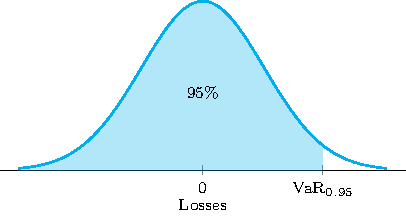
\includegraphics[width=0.5\textwidth]{figures/VaR}
	      % \caption{VaR$_{95\%}$ as the 95th percentile of the loss distribution.}
	      % \end{figure}

	\item CVaR (Conditional Value at Risk):\footnote{CVaR is also known
		      \emph{Expected Shortfall}.}

	      \begin{equation*}
		      \mathcal{R}(x) =\mbox{ES}_\alpha (x) = \mathbb{E}[L(x)|L(x)\geq \mbox{VaR}_\alpha(x)]
	      \end{equation*}
	      The CVaR, $\mbox{ES}_\alpha (x)$, is the expected value of loss, when it is grater than $\mbox{VaR}_\alpha$,
	      \begin{equation}
		      \mbox{ES}_\alpha(x) = \frac{1}{1-\alpha}\int_{\mbox{\footnotesize{VaR}}_\alpha(x)}^\infty u p(u)du
	      \end{equation}
	      where $p(u)$ is the probability density function of loss. CVaR quantifies the average loss above $\mbox{VaR}_\alpha$.

	      % The figure below shows the region where the CVaR is calculated.
	      % \begin{figure}[!h]
	      % \centering
	      % 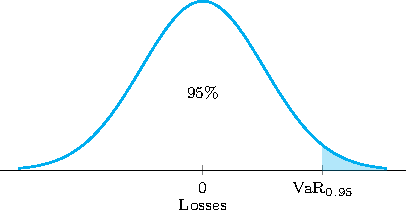
\includegraphics[width=0.5\textwidth]{figures/CVaR}
	      % \caption{Loss values used in CVaR calculation.}
	      % \end{figure}
\end{itemize}

While VaR answers the following question:

``\textit{What is the minimum portfolio loss in the $100(1-\alpha)$\% worst case scenarios}?''


CVaR answers the following question:

``\textit{What is the average loss of the portfolio in the $100(1-\alpha)$\% worst case scenarios?}''

\begin{remark}\normalfont \hspace{1cm}
	\begin{itemize}
		\item The standard deviation does not satisfy condition 4, however, this condition was defined with the perspective of banking system risk and is often ignored in case of portfolio construction.
		\item VaR is not a coherent risk measure as it does not satisfy condition 1. This is a problem because the portfolio’s risk may have be meaningful in this case.
		\item CVaR is a coherent risk measure.
	\end{itemize}
\end{remark}


Let us now assume that the returns are normally distributed, that is, $R\sim N(\mu,\sigma^2)$, where $\mu(x)=x^\top\mu$ and
$\sigma(x)=\sqrt{x^\top \Sigma x}$. Let $\phi(z) = \frac{1}{\sqrt{2\pi}}e^{-z^2/2}$ be the probability density function of Standard Normal Distribution and $\Phi(x) = \int_{-\infty}^{x}\phi(z) dz$
the standard normal accumulated density function.

By definition we have
$P\Big[L(x)\leq \mbox{VaR}_\alpha(x)\Big]=\alpha$, so
$P\Big[R(x)\leq -\mbox{VaR}_\alpha(x)\Big]=1-\alpha$, which standardizing
we have:
\[
	P\left[ \frac{R(x)-x^\top\mu}{\sqrt{x^\top \Sigma x}} \leq \frac{-\mbox{VaR}_\alpha(x)- x^\top\mu}{\sqrt{x^\top \Sigma x}}
		\right]=1-\alpha.
\]
Hence,
\[
	\frac{-\mbox{VaR}_\alpha(x)-x^\top\mu}{\sqrt{x^\top \Sigma x}}=\Phi^{-1}(1-\alpha)
\] and since $\Phi^{-1}(\alpha)=-\Phi^{-1}(1-\alpha)$, we have
\begin{equation}\label{eq:var2}
	\mbox{VaR}_\alpha(x)=-x^\top\mu+ \Phi^{-1}(\alpha)\sqrt{x^\top \Sigma x}.
\end{equation}

This is a special case of the standard deviation-based risk measure with $c = \Phi^{-1} (\alpha)$. It implies that the value-at-risk is a coherent and convex risk measure if the asset returns are normally distributed. The expression of the expected shortfall is:

\[
	\mbox{ES}_\alpha(x) = \frac{1}{1-\alpha}\int_{\mbox{VaR}_\alpha(x)}^\infty u p(u)du,
\] considering $p(u)$ the normal density function, we have that:
\[
	\mbox{ES}_\alpha(x) = \frac{1}{1-\alpha}\int_{-\mu(x)+ \sigma(x)\Phi^{-1}(\alpha)} ^\infty \frac{u}{\sigma(x)\sqrt{2\pi}} e^{-\frac{1}{2}\Big(\frac{u+\mu(x)}{\sigma (x)}\Big)^2} du,
\]

With the variable change
$t=\frac{u+\sigma(x)}{\sigma(x)}$, we obtain

\[
	\begin{aligned}
		\mbox{ES}_\alpha(x) & = \frac{1}{1-\alpha}\int_{\Phi^{-1}(\alpha)}^\infty (-\mu(x)+ \sigma(x)t) \frac{1}{\sqrt{2\pi}} e^{-t^2/2}dt \\
		                    & = -\frac{\mu(x)}{1-\alpha}[\Phi(t)]_{\Phi^{-1}(\alpha)}^\infty +
		\frac{\sigma(x)}{(1-\alpha)\sqrt{2\pi}}\int_{\Phi^{-1}(\alpha)}^\infty t e^{-t^2/ 2}dt                                             \\
		                    & =-\mu(x) + \frac{\sigma(x)}{(1-\alpha)\sqrt{2\pi}}\Big[-e^{-t^2/2} \Big] _{\Phi^{-1}(\alpha)}^\infty         \\
		                    & = -\mu(x) + \frac{\sigma(x)}{(1-\alpha)\sqrt{2\pi}}e^{-\frac{[\Phi^{-1}(\ alpha)]^2}{2}}
	\end{aligned}.
\]

So CVaR can be calculated by
\begin{equation}\label{eq:cvar2}
	\mbox{ES}_\alpha(x)=-x^\top \mu + \frac{\phi(\Phi^{-1}(\alpha))}{1-\alpha}\sqrt{x^ \top \Sigma x}.
\end{equation}
Like the value-at-risk, it is a standard deviation-based risk measure with $c ={\phi(\Phi^{-1}(\alpha))}/{(1-\alpha)}$
In the Gaussian world, different risk measures can be calculated using the expected return and volatility. Note by (\ref{eq:var2}) and (\ref{eq:cvar2}), that both Var and CVaR are the form $-\mu(x)+c\sigma(x)$. In general, we want a portfolio with positive returns, that is, $\mu(x)\geq0$. If the portfolio manager has very optimistic forecasts, component $\mu(x)$ may substantially reduce the risk measure. This explains why omitting the mean component is standard practice in the asset management industry.

\begin{example}\normalfont 
We consider three stocks $A$, $B$ and $C$ whose current prices are respectively $\$ 15.00$, $\$ 25.00$ and $\$ 30.00$. We assume that their expected returns are equal to $30$ bps\footnote{1 bps or one basis point is equivalent to
		0.01\% (the hundredth part of 1\%) or 0.0001 in decimal form.}, $50$ bps and $20$ bps on a daily basis and their daily volatilities are $3\%$, $2\%$, and $1\%$ respectively. The asset correlation matrix is given by
	\[
		\rho = \left(
		\begin{array}{rrr}
				1.00 & 0.40 & 0.15 \\
				0.40 & 1.00 & 0.60 \\
				0.15 & 0.60 & 1.00
			\end{array}
		\right)
	\]

	We consider a portfolio composed by $100$ stocks $A$, $200$ stocks $B$ and $100$ stocks $C$. The value of this portfolio is $\$ 9,500.00$, being $\$ 1,500.00$ invested in stock $A$, $\$ 5,000.00$ in stock $B$ and $\$ 3,000.00$ in stock $C$, therefore the weights of the stocks in this portfolio are $15.79\%$, $52.63\%$, and $31.58\%$ respectively, so $x=(0.1579;\;0.5263;\; 0.3158)$. The expected return on the portfolio is $\mu(x) = 30\times0.1579+50\times0.5263+20\times0.3158$, that is, $\mu(x) = 37$ bps. Using the relationship $\Sigma_{i,j}=\rho_{i,j}\sigma_1\sigma_j$ we find the covariance matrix
	\[
		\Sigma = \left(
		\begin{array}{llr}
				9.0 & 2.4 & 4.5 \\
				2.4 & 4.0 & 1.2 \\
				4.5 & 1.2 & 1.0
			\end{array}
		\right)\times10^{-4},
	\] since the volatility of portfolio is given by $\sigma^2(x) = x^\top \Sigma x$, we have that $\sigma(x) = 1.51\%$.

	Considering $\alpha = 0.99$, we have $\Phi^{-1}(0.99) = 2.325$ and
	$\phi(\Phi^{-1}(0.99))=\phi(2.325)=2.68\%$. Using the equations
	$(\ref{eq:var2})$ and $(\ref{eq:cvar2})$ we have

	\[
		\begin{aligned}
			\mathrm{VaR}_{99\%}(x) & = -0.37\% + 2.325 \times 1.51\% = 3.14\%              \\
			\mathrm{ES}_{99\%}(x)  & = -0.37\% + \frac{2.68}{0.01} \times 1.51\% = 3.68\%.
		\end{aligned}
	\]

	Risk can also be expressed in monetary terms, in this case,

	\[
		\begin{aligned}
			\mathrm{VaR}_{99\%}(x) & = 3.14\% \times \$ 9,500.00 = \$ 298.30  \\
			\mathrm{ES}_{99\%}(x)  & = 3.68\% \times \$ 9,500.00 = \$ 349.60.
		\end{aligned}
	\]
	According to the result of {\rm VaR}, in $99\%$ of the days, the loss will be less than $\$ 298.30$, however in the $1\%$ of the remaining days the {\rm VaR} does not measure how much great can be the loss, this is the role of {\rm CVaR} which indicates that the average loss will be $\$ 349.60$ on the worst $1\%$ days.
\end{example}




\chapter{Relative feasible inexact projections} \label{chap:SubInexProj}
\thispagestyle{empty}

%%%%%%%%%%%%%%%%%%%%%%%%%%%%%%%%%%%%%%%%%%%%%%%%%%%%%


In this chapter, we recall two concepts  of relative feasible inexact projections onto a closed and convex set, and  also  present  some  new properties of them which will be used throughout this work. These  concepts  of inexact projections were    introduced seeking to make the subproblem of computing the projections on the feasible  set more efficient;  see for example \cite{BirginMartinezRaydan2003,SalzoVilla2012,VillaSalzo2013}. Before presenting the  inexact projection concept that we will use, let us first recall the concept of exact projection with respect to a given  norm.  For that, {\it throughout this chapter we assume that $D\in {\cal D}_{\mu}$}.

\begin{definition} \label{def:exactProj}
	The {\it exact  projection of the point $v\in \mathbb{R}^{n}$ onto $C$ with respect to the norm $\| \cdot \| _{D}$}, denoted by  ${\cal P}_{C}^{D}(v)$, is  defined~by
	\begin{equation}\label{eq:exactM}
		{\cal P}_{C}^{D}(v):=\arg \min _{z\in C}\|z-v\|^2_{D}.
	\end{equation}
\end{definition}

The next result  characterizes  the exact projection, its  proof may be found in  \cite[Theorem 3.14]{BauschkeLivro2014}.

\begin{lemma} \label{pr:cham}
	Let $v, w \in {\mathbb R}^n$.  Then,  $w={\cal P}_{C}^{D}(v)$ if and only if  $w\in C$ and
	\begin{equation}\label{eq:exactA}
		\left\langle D(v-w), y-w\right\rangle \leq  0,
	\end{equation}

	for all $y \in C.$
\end{lemma}
\begin{remark}\normalfont
	It follows from Definition~\ref{def:exactProj} that $w={\cal P}_{C}^{D}(v)$ is the point of $C$ more close to $v$ with respect to the norm $\| \cdot \| _{D}$. On the other hand, by the Lemma \ref{pr:cham}, $w$ is the unique point of $C$ that for all $y\in C$ the angle $\theta$ among the vectors $v-w$ and $y-w$ is an obtuse angle. Figure~\ref{fig:exactProj} shows this fact considering the plane generated by points y, w and v.
\end{remark}\normalfont

\begin{figure}[!ht]
	\centering
	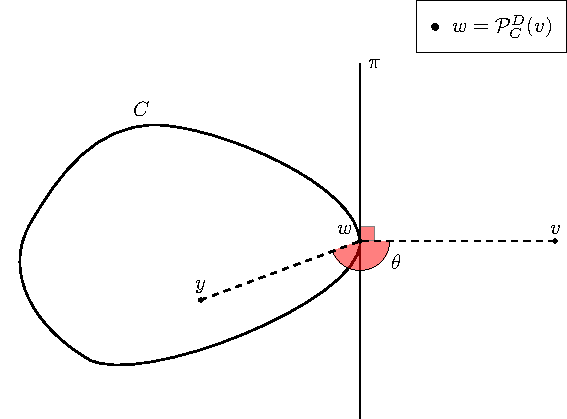
\includegraphics{figures/exactProj.pdf}
	\caption{Exact projection of the point $v$ onto $C$.}
	\label{fig:exactProj}
\end{figure}


\begin{remark}\normalfont \label{re:cproj}
	It follows from Lemma~\ref{pr:cham}  that $\|{\cal P}_{C}^{D}(v)-{\cal P}_{C}^{D}(u)\|_{D}\leq \|v-u\|_{D}$.  Moreover, since   $D\in {\cal D}_{\mu}$, by \eqref{eq:pnv}, we conclude that   ${\cal P}_{C}^{D}(\cdot)$ is Lipschitz continuous with constant $L=\mu$.   Furthermore,  if  $(D_k)_{k\in\mathbb{N}}\subset {\cal D}_{\mu}$,    $\lim_{k\to +\infty} z^{k} = \bar{z}$, and   $\lim_{k \to +\infty} D_{k} = \bar{D}$, then $\lim_{k \to +\infty}{\cal P}_{C}^{D_k}(z^{k})= {\cal P}_{C}^{\bar D}(\bar{z})$, see   \cite[Proposition~4.2]{CombettesVu2013}.
\end{remark}\

\section{The first feasible inexact projection}

In the following, we recall  the  concept of a  feasible inexact projection with respect to $\| \cdot \| _{D}$ relative to a fixed point.

\begin{definition} \label{def:InexactM}
	The {\it feasible inexact projection mapping, with respect to the norm $\| \cdot \|_{D}$,   onto $C$}  relative to a point  $u \in C$ and forcing parameter $\zeta\in (0, 1]$, denoted by ${\cal P}_{C,\zeta}^{D}(u,  \cdot): {\mathbb R}^n \rightrightarrows C$,  is the set-valued mapping defined as follows
	\begin{equation} \label{eq:Projwm}
		{\cal P}_{C,\zeta}^{D}(u, v) := \left\{w\in C:~ \|w-v\|_{D}^2\leq \zeta \| {\cal P}_{C}^{D}(v)-v\|_{D}^2+(1-\zeta)\|u-v\|_{D}^2 \right\}.
	\end{equation}
	Each point $w\in {\cal P}_{C,\zeta}^{D}(u, v) $ is called a  feasible inexact projection,  with respect to the norm $\| \cdot \|_{D}$,  of $v$ onto $C$ relative to $u$ and forcing parameter $\zeta\in (0, 1]$.
\end{definition}
\begin{remark}\normalfont
	It follows from Definition~\ref{def:InexactM} that ${\cal P}_{C,\zeta}^{D}(u, v)$ is a set generated by the intersection of $C$ and a sphere centered in $v$ and radius given by
	$$
		\zeta \| {\cal P}_{C}^{D}(v)-v\|_{D}^2+(1-\zeta)\|u-v\|_{D}^2.
	$$
	If $\zeta = 1$, then ${\cal P}_{C,1}^{D}(u, v) = \{{\cal P}_{C}^{D}(v)\}$ is the exact projection of $v$ onto $C$. However, when $\zeta$ is close to zero, the radius of sphere is close to $\|u-v\|_{D}$. The inexact condition appears when we consider points that do not minimize the distance from $C$ to $v$, contrary to property \eqref{eq:exactM}. This situation is illustrated in Figure~\ref{fig:martinezProj}.
\end{remark}\normalfont

\begin{figure}[H]
	\centering
	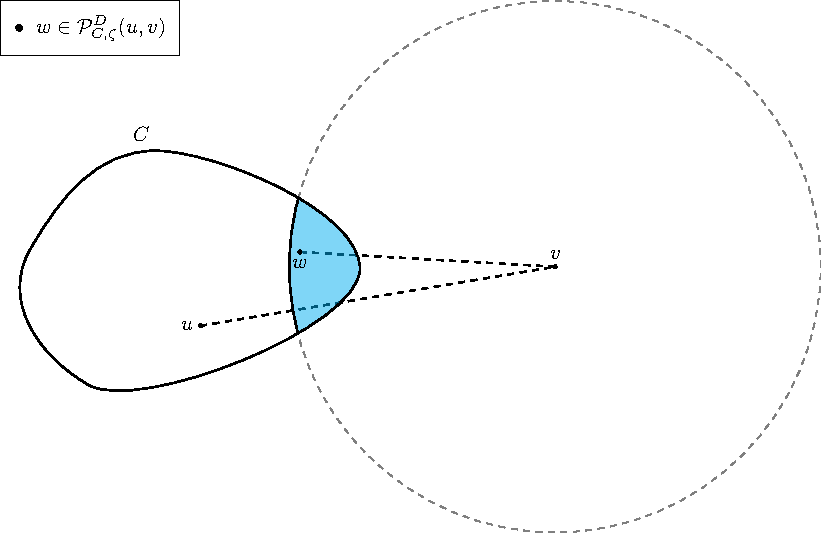
\includegraphics{figures/martinezProj.pdf}
	\caption{Feasible inexact projection of the point $v$ onto $C$.}
	\label{fig:martinezProj}
\end{figure}

In the following, we show that the definition given above is nothing more than a reformulation of the concept of  relative feasible inexact projection with respect to $\| \cdot \|_{D}$  introduced in  \cite{BirginMartinezRaydan2003}.
\begin{remark}\normalfont
	Let $u\in C$, $v\in \mathbb{R}^n$ and  $D$ be   an $n\times n$ positive definite matrix. Consider the quadratic  function $Q: \mathbb{R}^n \to \mathbb{R}$ defined by
	$$
		Q(z):=(1/2) \left\langle {D}(z-u),z-u\right\rangle +  \left \langle D(u-v), z-u \right\rangle.
	$$
	Thus,  letting  $\| \cdot \|_{D}$  be  the norm  defined by \eqref{def:normaD},  some algebraic manipulations   shows that
	\begin{equation} \label{eq:qppq}
		\|z-v\|^2_{D}= 2Q(z) +\|u-v\|^2_{D}.
	\end{equation}
	Hence,  \eqref{eq:qppq}  and \eqref{eq:exactM}  implies  that    ${\cal P}_{C}^{D}(v)=\arg \min _{z\in C}Q(z).$
	Let $\zeta\in (0, 1]$. Thus, by using \eqref{eq:qppq},  after some calculations,  we may see that  the following inexactness condition  introduced in \cite{BirginMartinezRaydan2003},
	$$
		w\in C, \qquad Q(w)\leq \zeta Q ( {\cal P}_{C}^{D}(v)) ,
	$$
	is  equivalent to find  $w\in C$ such that
	$$
		\|w-v\|_{D}^2\leq \zeta \| {\cal P}_{C}^{D}(v)-v\|_{D}^2+(1-\zeta)\|u-v\|_{D}^2,
	$$
	which corresponds to condition \eqref{eq:Projwm} in Definition~\ref{def:InexactM}.
\end{remark}\normalfont
The  concept of  feasible inexact projection  in Definition~\ref{def:InexactM}  provides  more latitude to   the usual  concept  of exact projection \eqref{eq:exactM}.  The next   remark makes  this more precise.
\begin{remark}\normalfont\label{rem: welldef}
	Let $\zeta$ be positive forcing parameter, $C\subset {\mathbb R}^n$ and $u\in C$ be as in Definition~\ref{def:InexactM}.  First of all note that  ${\cal P}_{C}^{D}( v) \in {\cal P}_{C,\zeta}^{D}(u, v)$. Therefore,  ${\cal P}_{C,\zeta}^{D}(u, v)\neq \varnothing$, for all $u\in C$ and $v\in {\mathbb R}^n$. Consequently, the set-valued mapping ${\cal P}_{C,\zeta}^{D}(u,  \cdot)$ as stated in \eqref{eq:Projwm} is well-defined.   Moreover,  for $\zeta=1$, we have ${\cal P}_{C,1}^{D}(u, v)=\{{\cal P}_{C}^{D}(v)\}$.
	In addition, if $\underline{\zeta}$ and $\bar{\zeta}$ are forcing parameters such that $0<\underline{\zeta}\leq \bar{\zeta}\leq 1$, then ${\cal P}_{C,\bar{\zeta}}^{D}(u, v) \subset {\cal P}_{C,\underline{\zeta}}^{D}(u, v)$.
\end{remark}\normalfont
\begin{lemma} \label{pr:condm}
	Let $v \in {\mathbb R}^n$, $u \in C$ and $w\in {\cal P}_{C,\zeta}^{D}(u, v)$. Then,
	$$
		\left\langle D(v-w), y-w\right\rangle \leq  \frac{1}{2} \|w-y\|_{D}^2 +   \frac{1}{2} \left[\zeta \| {\cal P}_{C}^{D}(v)-v\|_{D}^2+(1-\zeta)\|u-v\|_{D}^2 - \|y-v\|_{D}^2\right] ,   \qquad y \in C.
	$$
\end{lemma}
\begin{proof}
	Let  $y \in C$. Since   $  2\langle D(v-w), y-w\rangle = \|w-y\|_{D}^2 + \|w-v\|_{D}^2-\|v-y\|_{D}^2$,  using \eqref{eq:Projwm}  we have
	$2\langle D(v-w), y-w\rangle = \|w-y\|_{D}^2 + \zeta \| {\cal P}_{C}^{D}(v)-v\|_{D}^2+(1-\zeta)\|u-v\|_{D}^2-\|v-y\|_{D}^2$, which is equivalent to  the desired inequality.
\end{proof}

\section{The second feasible inexact projection}

Next, we recall a second  concept of relative  feasible inexact projection onto a closed convex set, see  \cite{Ademir_Orizon_Leandro2020, OrizonFabianaGilson2018}.  The definition  is as follows.
\begin{definition} \label{def:InexactProjC}
	The {\it feasible inexact projection mapping, with respect to the norm $\| \cdot \|_{D}$,  onto $C$} relative to $u \in C$ and forcing parameter $\gamma\geq 0$, denoted by ${\cal R}_{C,\gamma}^{D}(u, \cdot): {\mathbb R}^n \rightrightarrows C$,  is the set-valued mapping defined as follows
	\begin{equation} \label{eq:Projw}
		{\cal R}_{C,\gamma}^{D}(u, v):= \left\{w\in C:~\left\langle D(v-w), y-w \right\rangle \leq \gamma \|w-u\|_{D}^2, \quad \forall~ y \in C \right\}.
	\end{equation}
	Each point $w\in {\cal R}_{C,\gamma}^{D}(u, v)$ is called a feasible inexact projection,  with respect to the norm $\| \cdot \|_{D}$,  of $v$ onto $C$ relative to $u$ and forcing parameter $\gamma\geq 0$.
\end{definition}
The concept of  feasible inexact projection  in Definition~\ref{def:InexactProjC} also  provides  more latitude to  the usual concept  of exact projection. Next,  we present some remarks about this concept.
\begin{remark}\normalfont\label{rem: welldef}
	Let $\gamma\geq 0$ be a forcing parameter, $C\subset {\mathbb R}^n$ and $u\in C$ be as in Definition~\ref{def:InexactProjC}.
	For all $v\in {\mathbb R}^n$, it follows from \eqref{eq:Projw} and Lemma~\ref{pr:cham} that ${\cal R}_{C,0}^{D}(u, v)=\{{\cal P}_{C}^{D}(v)\}$ is the exact projection of $v$ onto $C$. Moreover, ${\cal P}_{C}^{D}(v)\in {\cal R}_{C,\gamma}^{D}(u, v)$ concluding  that ${\cal R}_{C, \gamma}(u, v)\neq \varnothing$, for all $u\in C$ and $v\in {\mathbb R}^n$. Consequently, the set-valued mapping ${\cal R}_{C,\gamma}^{D}(u, \cdot)$ as stated in \eqref{eq:Projw} is well-defined.
\end{remark}\normalfont

We show now a geometric interpretation for the inexact projection defined in Definition~\ref{def:InexactProjC}.
\begin{remark}\normalfont
	Let $C\subset \mathbb{R}^n$, $u\in C$, $v\in \mathbb{R}^n$, $w\in{\cal R}_{C,\gamma}^{D}(u, v)$ be as stated in Definition~\ref{def:InexactProjC} and $w_t = w+t(v-w)$, with $0\leq t <1$. It is easy to see that, for all $y\in C$,
	\begin{align*}
		\begin{aligned}
			% w_t - w & = t(v-w)        \\
			% v-w_t   & = (1-t)(v-w)    \\
			y-w_t & = y-w - t(v-w).
		\end{aligned}
	\end{align*}
\end{remark}
It follows from \eqref{eq:Projw} that $\left\langle D(v-w), y-w \right\rangle \leq \gamma \|w-u\|_{D}^2$, so we have
\begin{align*}
	\begin{aligned}
		\left\langle D(v-w_t), y-w_t \right\rangle & = (1-t)\left\langle D(v-w), y-w \right\rangle - t(1-t)\|v-w\|_D^{2} \\
		                                           & \leq  (1-t)\left[ \gamma \|w-u\|_D^2 - t\|v-w\|_D^2 \right].
	\end{aligned}
\end{align*}
Since $0\leq t<1$,
$$
	\|w_t-w\|_D^2 = t^2 \|v-w\|_D^2 \leq t\|v-w\|_D^2,
$$
if
\begin{equation}\label{eq:condProj}
	\gamma \|w-u\|_D^2 \leq \|w_t-w\|_D^2
\end{equation}
then $\left\langle D(v-w_t), y-w_t \right\rangle\leq 0$. In this case the inexact condition appears considering that there is $w_t$ between $w$ and $v$ that satisfies \eqref{eq:condProj} and consequently the condition \eqref{eq:exactA}.  This situation is illustrated in Figure~\ref{fig:condProj1}.


\begin{figure}[H]
	%\begin{adjustwidth}{2.2cm}{2.2cm}
	\begin{subfigmatrix}{2}
		\subfigure[Geometric interpretation.]{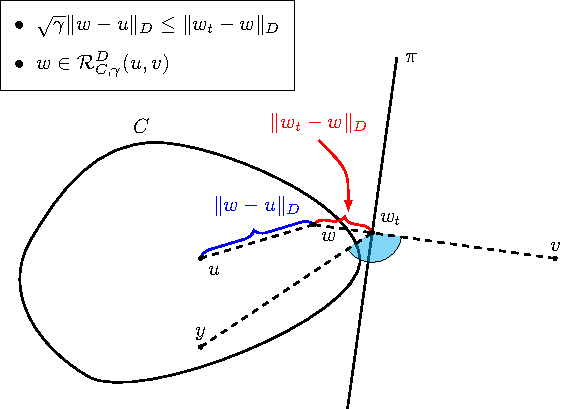
\includegraphics{figures/condProj1.pdf}}
		\subfigure[Example of ${\cal R}_{C,\gamma}^{D}(u, v)$.]{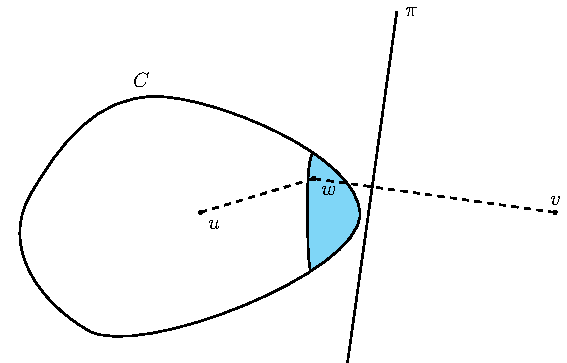
\includegraphics{figures/condProj2.pdf}}
	\end{subfigmatrix}
	\caption{Geometric interpretation of projection ${\cal R}_{C,\gamma}^{D}(u, v)$.}
	\label{fig:condProj1}
	%\end{adjustwidth}
\end{figure}
In the following we presents some examples of regions given by inexact projection ${\cal R}_{C,\gamma}^{D}(u, v)$. Note that the projection ${\cal R}_{C,\gamma}^{D}(u, v)$ gets smaller as $u$ gets closer to $w$.
\begin{figure}[H]
	%\begin{adjustwidth}{2.2cm}{2.2cm}
	\begin{subfigmatrix}{3}
		\subfigure[]{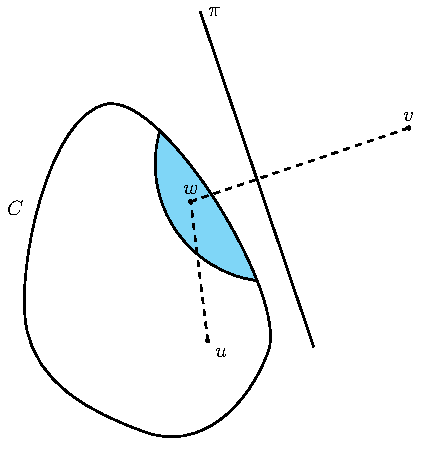
\includegraphics{figures/condProj3.pdf}}
		\subfigure[]{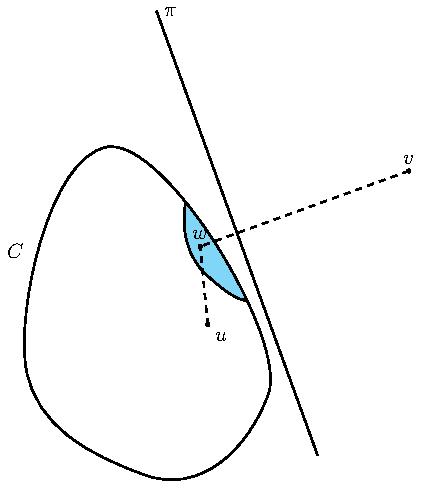
\includegraphics{figures/condProj4.pdf}}
		\subfigure[]{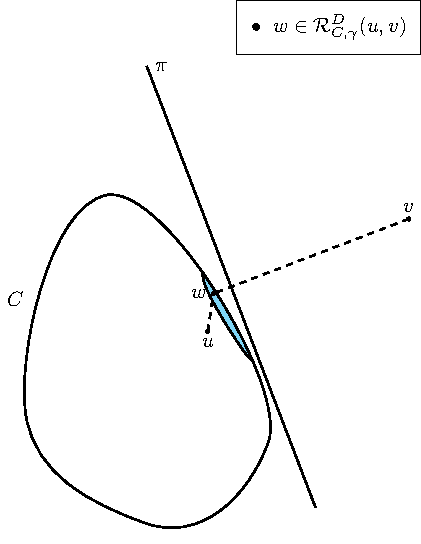
\includegraphics{figures/condProj5.pdf}}
	\end{subfigmatrix}
	\caption{Examples of regions given by inexact projection ${\cal R}_{C,\gamma}^{D}(u, v)$.}
	\label{fig:baseline}
	%\end{adjustwidth}
\end{figure}
The next example shows the behavior of the projection ${\cal R}_{C,\gamma}^{D}(u, v)$ when the set $C$ has a vertice and some flat parts.
\begin{figure}[H]
	%\begin{adjustwidth}{2.2cm}{2.2cm}
	\begin{subfigmatrix}{3}
		\subfigure[]{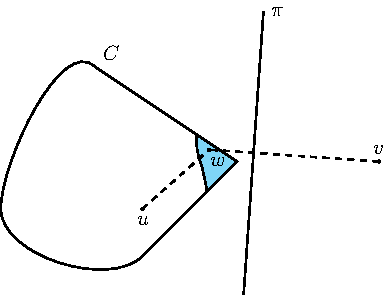
\includegraphics[width=0.3\linewidth]{figures/condProj6.pdf}}
		\subfigure[]{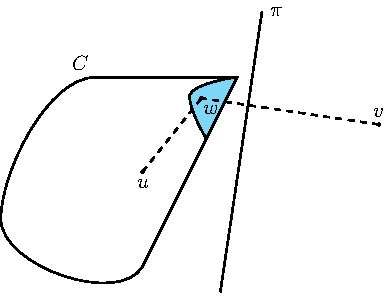
\includegraphics[width=0.3\linewidth]{figures/condProj7.pdf}}
		\subfigure[]{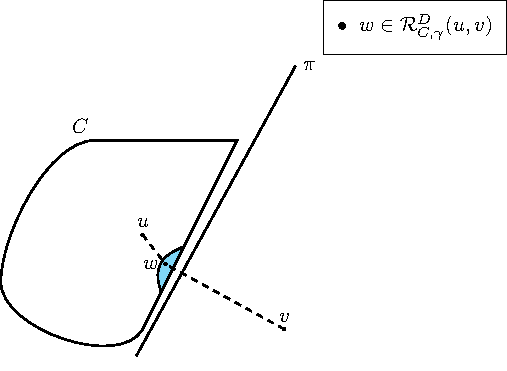
\includegraphics[width=0.38\linewidth]{figures/condProj8.pdf}}
	\end{subfigmatrix}
	\caption{Examples of regions given by inexact projection ${\cal R}_{C,\gamma}^{D}(u, v)$.}
	\label{fig:baseline}
	%\end{adjustwidth}
\end{figure}

The  next lemma is a variation of \cite[Lemma 6]{Reiner_Orizon_Leandro2019}.  It will allow to relate Definitions~\ref{def:InexactM} and \ref{def:InexactProjC}.
\begin{lemma} \label{pr:cond}
	Let $v \in {\mathbb R}^n$, $u \in C$, $\gamma \geq 0$ and $w\in {\cal R}_{C,\gamma}^{D}(u, v)$. Then,  for all $0 \leq \gamma <1/2$, the holds
	$$
		\displaystyle \|w-x\|_{D}^2 \leq \|x-v\|_{D}^2 + \frac{2\gamma}{1-2\gamma}\|u-v\|_{D}^2- \frac{1}{1-2\gamma}\|w-v\|_{D}^2, \qquad \forall x \in C.
	$$
\end{lemma}
\begin{proof}
	First note that $\|w-x\|_{D}^2 = \|x-v\|_{D}^2 - \|w-v\|_{D}^2 + 2 \langle D(v-w), x-w \rangle$. Since $w \in {\cal R}_{C,\gamma}^{D}(u, v)$ and $x \in C$, combining the last equality with \eqref{eq:Projw}, we obtain
	\begin{equation} \label{eq:fg}
		\|w-x\|_{D}^2 \leq \|x-v\|_{D}^2 - \|w-v\|_{D}^2  + 2\gamma \|w-u\|_{D}^2.
	\end{equation}
	On the other hand, we also have $\|w-u\|_{D}^2=\|u-v\|_{D}^2 - \|w-v\|_{D}^2 +  2 \langle D(v-w), u-w \rangle$. Due to $w\in {\cal R}_{C,\gamma}^{D}(u, v)$ and $u \in C$, using \eqref{eq:Projw} and considering that  $0 \leq \gamma < 1/2$, we have
	$$
		\|w-u\|_{D}^2 \leq \frac{1}{1-2\gamma}\|u-v\|_{D}^2 - \frac{1}{1-2\gamma} \|w-v\|_{D}^2.
	$$
	Therefore, substituting the last inequality into   \eqref{eq:fg}, we obtain the  desired inequality.
\end{proof}

\section{The relationship among feasible inexact projections}

In the following  lemma, we present a  relationship between   Definitions~\ref{def:InexactM} and \ref{def:InexactProjC}.
\begin{lemma} \label{pr:condrip}
	Let $v \in {\mathbb R}^n$, $u \in C$, $\gamma \geq 0$  and $\zeta\in (0, 1]$.  If  $0 \leq \gamma <1/2$ and $\zeta=1-2\gamma$, then
	$$
		{\cal R}_{C,\gamma}^{D}(u, v) \subset {\cal P}_{C,\zeta}^{D}(u, v).
	$$
\end{lemma}
\begin{proof}
	Let $w\in {\cal R}_{C,\gamma}^{D}(u, v)$. Applying Lemma~\ref{pr:cond} with  $x={\cal P}_{C}^{D}(v)$ we have
	$$
		\|w-{\cal P}_{C}^{D}(v)\|_{D}^2 \leq \|v-{\cal P}_{C}^{D}(v)\|_{D}^2 + \frac{2\gamma}{1-2\gamma}\|u-v\|_{D}^2- \frac{1}{1-2\gamma}\|w-v\|_{D}^2,
	$$
	After some algebraic manipulations in the last inequality we obtain that
	$$
		\|w-v\|_{D}^2 \leq (1-2\gamma)\|v-{\cal P}_{C}^{D}(v)\|_{D}^2 + 2\gamma\|u-v\|_{D}^2- (1-2\gamma)\|w-{\cal P}_{C}^{D}(v)\|_{D}^2.
	$$
	Therefore, considering that  $0 \leq \gamma <1/2$ and $\zeta=1-2\gamma$, the result follows from Definition~\ref{def:InexactM}.
\end{proof}

\begin{remark}\normalfont \label{re:ni}
	Under the conditions of  Lemma \ref{pr:condrip}, there exists  $0 \leq \gamma <1/2$ and $\zeta=1-2\gamma$ such that ${\cal P}_{C,\zeta}^{D}(u, v)  \nsubseteq    {\cal R}_{C,\gamma}^{D}(u, v)$. Indeed,  let $\gamma=3/8$, $\zeta=1/4$,  and ${\bar w}=\frac{1}{2}({\cal P}_{C}^{D}(v)+u)$, then
	$$
		\displaystyle\|{\bar w}-v\|_D^2=\frac{1}{4}\| {\cal P}_{C}^{D}(v)-v\|_D^2 + \frac{1}{4}\|u-v\|_D^2 +\frac{1}{2} \langle D( {\cal P}_{C}^{D}(v) -v), u-v \rangle.
	$$
	Since  $ {\cal P}_{C}^{D}(v)$ is the exact projection of $v$,  we have   $\displaystyle\langle D( {\cal P}_{C}^{D}(v) -v), u-v \rangle \leq \|u-v\|_D^2$. Combining this inequality with  the last equality and Definition~\ref{def:InexactM}, we conclude that ${\bar w}\in {\cal P}_{C,\zeta}^{D}(u, v)$. Now,  letting $w_t=t{\cal P}_{C}^{D}(v)+ (1-t){\bar w}$  with $0<t<1$, after some algebraic  manipulations  we have
	$$
		\langle D(v-{\bar w}), w_t-{\bar w} \rangle=t\| {\bar w}-u\|_D^2 - \frac{t}{2} \langle D( v- {\cal P}_{C}^{D}(v)) , u-{\cal P}_{C}^{D}(v)  \rangle.
	$$
	Thus, it follows from Lemma~\ref{pr:cham} that $\displaystyle \langle D(v-{\bar w}), w_t-{\bar w} \rangle\geq t\| {\bar w}-u\|_D^2 $.  Hence,  taking  $t>3/8$ we conclude that ${\bar w}\not\in{\cal R}_{C,\gamma}^{D}(u, v)$.  Therefore, considering that ${\bar w}\in {\cal P}_{C,\zeta}^{D}(u, v)$, the statement follows.
\end{remark}\normalfont
It follows from Remark~\ref{re:ni} that, in general,  ${\cal P}_{C,\zeta}^{D}(u, v)  \nsubseteq    {\cal R}_{C,\gamma}^{D}(u, v)$. However, whenever $C$ is a bounded set,  we will show  that   for each  fixed  $0 \leq \gamma <1/2$  there exist $0 < \zeta  <1$ such that    ${\cal P}_{C,\zeta}^{D}(u, v)  \subseteq    {\cal R}_{C,\gamma}^{D}(u, v)$. For that, we first need the next lemma.
\begin{lemma} \label{le:epsi}
	Let $v \in {\mathbb R}^n$, $u \in C$ and $0<\gamma < 1/2$. Assume that $C$ is a bounded set and take
	\begin{equation} \label{eq:epsi}
		0<\varepsilon < \frac{\gamma \|u-\mathcal{P}_C^D(v)\|_D^2}{1-\gamma+\|v-\mathcal{P}_C^D(v)\|_D+ 2	\gamma\|u-\mathcal{P}_C^D(v)\|_D+\mbox{\normalfont diam}C },
	\end{equation}
	where $\mbox{\normalfont diam}C$ denotes the diameter of $C$. Then, $\{w\in C: ~ \|w-\mathcal{P}_C^D(v)\|_D\leq \varepsilon\}\subset\mathcal{R}_{C,\gamma}^D(u, v)\}$.
\end{lemma}
\begin{proof}
	Take $\varepsilon$ satisfying \eqref{eq:epsi} and $w\in C$ such that  $\|w-\mathcal{P}_C^D(v)\|_D\leq \varepsilon$ . For all $z\in C$, we have
	\begin{multline*}
		\langle D(v-w), z-w \rangle = \langle D(v-\mathcal{P}_C^D(v)),z-\mathcal{P}_C^D(v) \rangle + \langle D(v-\mathcal{P}_C^D(v)), \mathcal{P}_C^D(v) -w \rangle\\
		+ \langle D(\mathcal{P}_C^D(v) - w), z- \mathcal{P}_C^D(v) \rangle +\| \mathcal{P}_C^D(v)-w\|_D^2.
	\end{multline*}
	Using Lemma~\ref{pr:cham},  we have $\langle D(v-\mathcal{P}_C^D(v)),z-\mathcal{P}_C^D(v) \rangle\leq 0$. Thus, the last equality becomes
	$$
		\langle D(v-w), z-w \rangle \leq \langle D(v-\mathcal{P}_C^D(v)), \mathcal{P}_C^D(v) -w \rangle + \langle D(\mathcal{P}_C^D(v) - w), z- \mathcal{P}_C^D(v) \rangle +\| \mathcal{P}_C^D(v)-w\|_D^2.
	$$
	By using Cauchy-Schwarz inequality, we conclude from the last inequality that
	$$
		\langle D(v-w), z-w \rangle \leq  \|w-\mathcal{P}_C^D(v) \|_D\left(\|v-\mathcal{P}_C^D(v)\|_D+ \|z- \mathcal{P}_C^D(v)\|_D\right) +\|w-\mathcal{P}_C^D(v)\|_D^2.
	$$
	Since $\|w-\mathcal{P}_C^D(v)|_D\leq \varepsilon$ and $ \|z- \mathcal{P}_C^D(v)\|_D\leq \mbox{diam} C$, the last inequality implies that
	\begin{equation}\label{eq:diam1}
		\langle D(v-w), z-w \rangle \leq \varepsilon \left(\|v-\mathcal{P}_C^D(v)\|_D+\mbox{diam}C\right)+\varepsilon^2,
	\end{equation}
	On the other hand, if $\varepsilon$ satisfies \eqref{eq:epsi} then
	$$
		\varepsilon \left( 1-\gamma+\|v-\mathcal{P}_C^D(v)\|_D+ \mbox{diam} C\right) + \gamma \varepsilon^2 <
		\gamma\|u-\mathcal{P}_C^D(v)\|_D^2-2	\gamma\varepsilon\|u-\mathcal{P}_C^D(v)\|_D +\gamma\varepsilon^2,
	$$
	hence
	$
		\varepsilon \left( 1-\gamma+\|v-\mathcal{P}_C^D(v)\|_D+ \mbox{diam} C\right) + \gamma \varepsilon^2 < \gamma\left(\|u-\mathcal{P}_C^D(v)\|_D-\varepsilon\right)^2.
	$
	Since $\gamma, \varepsilon<1$, we have  $\varepsilon^2 < \varepsilon(1-\gamma) + \gamma \varepsilon^2$ and we may conclude that
	$$
		\varepsilon \left( \|v-\mathcal{P}_C^D(v)\|_D+ \mbox{diam} C\right) + \varepsilon^2 <
		\gamma\left(\|u-\mathcal{P}_C^D(v)\|_D-\varepsilon\right)^2.
	$$
	It follows from \eqref{eq:diam1} that
	\begin{equation}\label{eq:diam2}
		\langle D(v-w), z-w \rangle \leq \gamma\left(\|u-\mathcal{P}_C^D(v)\|_D-\varepsilon\right)^2.
	\end{equation}
	Using again that $\|w-\mathcal{P}_C^D(v)|_D\leq \varepsilon$ and the triangular inequality, we have
	$$
		0<\|u-\mathcal{P}_C^D(v)\|_D -\varepsilon \leq \|u-\mathcal{P}_C^D(v)\|_D -\|w-\mathcal{P}_C^D(v)\|_D \leq \|u-w\|_D.
	$$
	Hence,   taking into account  \eqref{eq:diam2}, we conclude that $	\langle D(v-w), z-w \rangle \leq \gamma\|u-w\|_D^2$. Therefore, it follows from Definition~\ref{def:InexactProjC} that    $w\in\mathcal{R}_{C,\gamma}^D(u, v)$.
\end{proof}
\begin{proposition} \label{le:pcr}
	Let $v \in {\mathbb R}^n$, $u \in C$ and assume that $C$ is a bounded set. Then, for each $0<\gamma < 1/2$,     there exist $0 < \zeta  <1$ such that    ${\cal P}_{C,\zeta}^{D}(u, v)  \subseteq    {\cal R}_{C,\gamma}^{D}(u, v)$.
\end{proposition}
\begin{proof}
	It follows from Lemma~ \ref{le:epsi}  that given $0<\gamma<1/2$ there exists $\varepsilon>0$ such that,  for all $w\in C$  with $\|w-\mathcal{P}_C^D(v)\|\leq \varepsilon$, we have  $w\in\mathcal{R}_\gamma^D(v)$. Otherwise,  we may see in (\ref{eq:Projwm}), when $\zeta\to 1$, the diameter of $C\cap{\cal P}_{C,\zeta}^{D}(u, v)$ tends to zero, then there exists  $\zeta$ close to 1 such that $\mbox{diam}(C\cap{\cal P}_{C,\zeta}^{D}(u, v))<\varepsilon/2$, and ${\cal P}_{C,\zeta}^{D}(u, v) \subset {\cal R}_{C,\gamma}^{D}(u, v)$.
\end{proof}

Next, we present  important properties of  inexact projections,  it  will be useful in  the sequel.
\begin{lemma} \label{Le:ProjProperty}
	Let $x \in C$, $\alpha > 0$ and  $z(\alpha) = x-\alpha D^{-1} \nabla f(x)$. Take $w(\alpha) \in  {\cal P}_{C,\zeta}^{D}(x, z(\alpha))$ with $\zeta\in (0, 1]$. Then,
	\begin{itemize}
		\item[(i)] $\displaystyle \langle \nabla f(x), w(\alpha) - x\rangle \leq -\frac{1}{2\alpha} \|w(\alpha) -x\|_{D}^2 +   \frac{\zeta}{2\alpha} \left[\| {\cal P}_{C}^{D}(z(\alpha))-z(\alpha)\|_{D}^2 - \|x-z(\alpha)\|_{D}^2\right]$;
		\item[(ii)] the point $x$ is stationary for problem \eqref{eq:OptP} if and only if $x \in {\cal P}_{C,\zeta}^{D}(x, z(\alpha))$;
		\item[(iii)] if  $x \in C$ is a nonstationary point for problem \eqref{eq:OptP}, then $\Big\langle \nabla f(x), w(\alpha) - x \Big\rangle < 0$. Equivalently, if there exists ${\bar \alpha}>0$ such that $\Big\langle \nabla f(x), w({\bar \alpha}) - x \Big\rangle \geq 0$, then $x$ is stationary for problem \eqref{eq:OptP}.
	\end{itemize}
\end{lemma}
\begin{proof}
	Since $w(\alpha) \in  {\cal P}_{C,\zeta}^{D}(x, z(\alpha))$, applying Lemma~\ref{pr:condm} with   $w=w(\alpha)$, $v=z(\alpha)$, $y=x$,  and $u=x$, we conclude,  after some algebraic manipulations,  that
	$$
		\left\langle D(z(\alpha)-w(\alpha)), x-w(\alpha) \right\rangle \leq 	\frac{1}{2} \|w(\alpha) -x\|_{D}^2 +   \frac{\zeta}{2} \left[\| {\cal P}_{C}^{D}(z(\alpha))-z(\alpha)\|_{D}^2 - \|x-z(\alpha)\|_{D}^2\right].
	$$
	Substituting  $z(\alpha) = x-\alpha \nabla f(x)$ in the left hand side of the last inequality,   some manipulations yield the inequality of item $(i)$.  For proving item $(ii)$, we first assume that $x$ is stationary for problem \eqref{eq:OptP}. In this case, \eqref{eq:StatPoint} implies that $\langle \nabla f(x), w(\alpha)-x \rangle \geq 0$. Hence,  due to $\|{\cal P}_{C}^{D}(z(\alpha))-z(\alpha)\|_{D}\leq  \|x-z(\alpha)\|_{D}$,   item $(i)$ implies
	$$
		\frac{1}{2\alpha} \|w(\alpha) -x\|_{D}^2 \leq    \frac{\zeta}{2\alpha} \left[\| {\cal P}_{C}^{D}(z(\alpha))-z(\alpha)\|_{D}^2 - \|x-z(\alpha)\|_{D}^2\right]\leq 0.
	$$
	Since $\alpha > 0$ and  $\zeta\in (0, 1]$, the last inequality  yields  $w(\alpha) = x$.  Therefore, $x \in {\cal P}_{C,\zeta}^{D}(x, z(\alpha))$. Reciprocally, if  $x \in {\cal P}_{C,\zeta}^{D}(x, z(\alpha))$, then Definition~\ref{def:InexactM} implies that
	$$
		\|x-z(\alpha)\|_{D}^2\leq \zeta \| {\cal P}_{C}^{D}(z(\alpha))-z(\alpha)\|_{D}^2+(1-\zeta)\|x-z(\alpha)\|_{D}^2.
	$$
	Hence, $0\leq \zeta\left( \| {\cal P}_{C}^{D}(z(\alpha))-z(\alpha)\|_{D}^2-(\|x-z(\alpha)\|_{D}^2\right)$. Considering that  $\zeta\in (0, 1]$ we have
	$$
		\|x-z(\alpha)\|_{D}\leq\| {\cal P}_{C}^{D}(z(\alpha))-z(\alpha)\|_{D}.
	$$
	Thus, due to  exact projection  with respect to the norm $\| \cdot \| _{D}$   be unique and $z(\alpha) = x-D^{-1} \alpha \nabla f(x)$,   we have    ${\cal P}_{C}^{D}( x-\alpha D^{-1} \nabla f(x))=x$. Hence, $x$ is the  solution of the constrained optimization problem $  \min _{y\in C}  \|y-z(\alpha)\| ^{2}_{D}$,
	which taking into account that  $\alpha > 0$ implies \eqref{eq:StatPoint}. Therefore, $x$ is stationary point for problem \eqref{eq:OptP}. Finally, to prove item $(iii)$, take $x$ a nonstationary point for problem \eqref{eq:OptP}. Thus, by item $(ii)$, $x \notin  {\cal P}_{C,\zeta}^{D}(x, z(\alpha))$ and taking into account that $w(\alpha) \in  {\cal P}_{C,\zeta}^{D}(x, z(\alpha))$, we conclude that $x \neq w(\alpha)$. Since $\|{\cal P}_{C}^{D}(z(\alpha))-z(\alpha)\|_{D}\leq  \|x-z(\alpha)\|_{D}$, $\alpha > 0$ and $\zeta\in (0, 1]$, it follows from item $(i)$ that $\Big\langle \nabla f(x), w(\alpha) - x \Big\rangle < 0$ and the first sentence is proved. Finally, note that the second sentence is the contrapositive of the first sentence.
\end{proof}

Finally, it is worth mentioning that Definitions~\ref{def:InexactM} and \ref{def:InexactProjC}, introduced respectively in \cite{BirginMartinezRaydan2003} and \cite{OrizonFabianaGilson2018},  are relative inexact  concepts, while the concept introduced in \cite{SalzoVilla2012,VillaSalzo2013} is absolute.



%%%%%%%%%%%%%%%%%%%%%%%%%%%%%%%%%%
\section{Practical computation of  inexact projections} \label{sec:pcip}

In this section,  for a given  $v\in {\mathbb R}^n$ and   $u \in C$, we discuss how to calculate a  point  $w \in C$ belonging to  ${\cal P}_{C, \zeta}^{D}(u,v)$ or ${\cal R}_{C, \gamma}^{D}(u,v)$.  We recall that  Lemma~\ref{pr:condrip} implies that ${\cal P}_{C, \zeta}^{D}(u,v)$ has  more latitude than ${\cal R}_{C, \gamma}^{D}(u,v)$, i.e., ${\cal R}_{C, \gamma}^{D}(u,v) \subset {\cal P}_{C, \zeta}^{D}(u,v)$.

We begin our discussion by showing how a point $w\in {\cal P}_{C, \zeta}^{D}(u,v)$ may be calculated  without knowing the point ${\cal P}_{C}^{D}(v)$.   Considering that this discussion has already been covered in \cite[Section~3,  Algorithm 3.1]{BirginMartinezRaydan2003},  we will limit ourselves to giving a general idea of how this task is carried out; see also \cite[Section~5.1]{Bonettini2016}.   The idea is to use an external procedure capable of computing two  sequences  $(c_\ell)_{\ell\in\mathbb{N}}\subset \mathbb{R}$  and   $(w^\ell)_{\ell\in\mathbb{N}}\subset C$ satisfying the following  conditions
\begin{equation}\label{def:cl}
	c_\ell \leq \|{\cal P}_{C}^{D}(v)-v\|_D^2,\quad  \forall\ell\in\mathbb{N}, \qquad \qquad \lim_{\ell \to +\infty} c_\ell = \|{\cal P}_{C}^{D}(v)-v\|_D^2, \qquad \quad   \lim_{\ell\to +\infty} w^\ell = {\cal P}_{C}^{D}(v).
\end{equation}
In this case,   if  $v\notin C$, then   we have $ \|{\cal P}_{C}^{D}(v)-v\|_D^2- \|u-v\|_D^2<0$. Hence,   given an arbitrary $ \zeta\in (0,1)$,  the second condition in \eqref{def:cl} implies  that   there exists $\hat{\ell}$ such that
$$
	\|{\cal P}_{C}^{D}(v)-v\|_D^2- \|u-v\|_D^2< \zeta (c_{\hat{\ell}}- \|u-v\|_D^2).
$$
Moreover, by using the last condition in \eqref{def:cl}, we conclude that   there exists $\bar{\ell}>\hat{\ell}$ such that
\begin{equation}\label{def:clsc}
	\|w_{\bar{\ell}}-v\|_D^2- \|u-v\|_D^2< \zeta (c_{\bar{\ell}}- \|u-v\|_D^2),
\end{equation}
which using   the inequality  in \eqref{def:cl} yields
$$
	\|w_{\bar{\ell}}-v\|_D^2<  \zeta \|{\cal P}_{C}^{D}(v)-v\|_D^2  +(1-\zeta) \|u-v\|_D^2.
$$
Hence, Definition~\ref{def:InexactM} implies that  $w_{\bar{\ell}}\in  {\cal P}_{C, \zeta}^{D}(u, v)$.   Therefore,   \eqref{def:clsc}  may be used as a stopping criterion to compute  a  feasible inexact projection,  with respect to the norm $\| \cdot \|_{D}$,  of $v$ onto $C$ relative to $u$ and forcing parameter $\zeta\in (0, 1]$. For instance,  it follows from   \cite[Theorem~3.2, Lemma~3.1]{BirginMartinezRaydan2003} (see also \cite{BirginRaydan2005}) that  such sequences  $(c_\ell)_{\ell\in\mathbb{N}}\subset \mathbb{R}$  and   $(w^\ell)_{\ell\in\mathbb{N}}\subset C$  satisfying  \eqref{def:cl}  may be computed by using   {\it Dykstra's algorithm} \cite{Dykstra1986, Dykstra1983}, whenever  $D$ is the identity matrix  and the set $C=\cap_{i=1}^p C_i$, where $C_i$ are closed and convex sets and the exact projection  ${\cal P}_{C_i}^{D}(v)$ is easy to obtain, for all $i=1,\dots,p$.

We end this section by discussing how to compute a point $w\in{\cal R}_{C, \gamma}^{D}(u,v)$. For that, we apply the classical {\it Frank-Wolfe method}, also known as {\it conditional gradient method},   to minimize the function  $\psi(z) := \|z - v\|^2/2$ onto  the constraint set $C$ with  a suitable  stop criteria depending  of $u\in C$ and $\gamma \in (0, 1]$, see  \cite{BeckTeboulle2004, Jaggi2013}.  To state the method  we assume the existence of a linear optimization oracle (or simply LO oracle) capable of minimizing linear functions over the constraint set $C$,   which is assumed to be  compact. The   Frank-Wolfe method is  formally stated as follows.

\begin{algorithm}[H]
	\begin{description}
		\item[Input:]  $D\in {\cal D}_{\mu}$,  $\gamma \in (0, 1]$,  $v\in {\mathbb R}^n$ and   $u \in C$.
		\item[ Step 0.] Let $w^0\in  C$ and  set $\ell \gets 0$.
		\item[ Step 1.] Use a LO oracle to compute an optimal solution $z^\ell$ and the optimal value $s_{\ell}^*$ as
			\begin{equation}\label{eq:CondG_{C}}
				z^\ell \in  \arg\min_{z \in  C} \,\langle w^\ell-v, ~z-w^\ell\rangle,  \qquad s_{\ell}^*:=\langle  w^\ell-v, ~z^\ell-w^\ell \rangle.
			\end{equation}
			If $-s^*_{\ell}\leq \gamma \|w^{\ell}-u\|_{D}^2$, then define $w:=w^\ell$ and {\bf stop}.
		\item[ Step 2.]  Compute $\alpha_\ell$ and $w_{\ell+1}$ as
			\begin{equation}\label{eq:step size}
				w_{\ell+1}:=w^\ell+ \alpha_\ell(z^\ell-w^\ell), \qquad {\alpha}_\ell: =\min\left\{1, -s^*_{\ell}/\|z^\ell-w^\ell\|^2 \right\}.
			\end{equation}
			Set $\ell\gets \ell+1$, and go to Step~1.
		\item[Output:]   $w:=w^\ell$.
	\end{description}
	\caption{Frank-Wolfe  method to compute $w\in {\cal R}_{C, \gamma}^{D}(u,v)$}
	\label{Alg:CondG}
\end{algorithm}

Let us  describe the main features of  Algorithm~\ref{Alg:CondG}, i.e.,  the  Frank-Wolfe method applied to the problem $\min_{z \in C}\psi(z)$.   In this case,  \eqref{eq:CondG_{C}} is equivalent to $s_{\ell}^*:=\min_{z \in C}\langle \psi'(w^\ell) ,~z-w^\ell\rangle$. Since $\psi$ is convex, we have
$$
	\psi(z)\geq \psi(w^\ell) + \langle \psi'(w^\ell) ,~z-w^\ell\rangle\geq    \psi(w^\ell)  +   s_{\ell}^*,
$$
for all $z\in C$. Define  $ w_*:=\arg \min_{z \in C}\psi(z)$ and  $\psi^*:= \min_{z \in C}\psi(z)$. Letting $z= w_*$ in the last inequality,  we obtain $$\psi(w^\ell)\geq \psi^* \geq \psi(w^\ell)  +   s_{\ell}^*,$$ which implies that $s_{\ell}^*< 0$ whenever $\psi(w^\ell)\neq \psi^*$. Thus, we conclude that
$$
	-s_{\ell}^*=\langle  v-w^\ell, ~z^\ell-w^\ell \rangle>0\geq  \langle  v-w_*, ~z-w_* \rangle,
$$
for all~$z\in C$.   Therefore, if  Algorithm~\ref{Alg:CondG} computes  $w^\ell \in C$ satisfying $-s_{\ell}^*\leq  \gamma \|w^{\ell}-u\|_{D}^2$, then the method terminates. Otherwise, it computes the step size $\alpha_\ell = \arg\min_{\alpha \in [0,1]} \psi(w^\ell + \alpha(z^\ell - w^\ell))$  using exact minimization.  Since $z^\ell$, $w^\ell \in C$  and $C$ is convex, we conclude from  \eqref{eq:step size}  that $w_{\ell+1} \in C$, thus  Algorithm~\ref{Alg:CondG}  generates a sequence in $C$.  Finally,   \eqref{eq:CondG_{C}} implies that  $\langle  v-w^\ell, ~z-w^\ell\rangle\leq -s_{\ell}^*$, for all  $ z\in C$.  Considering that   \cite[Proposition A.2]{BeckTeboulle2004}  implies that $\lim_{\ell \to +\infty}s_{\ell}^*=0$ and taking into account   the  stopping criteria     $-s_{\ell}^*\leq \gamma \|w^{\ell}-u\|_{D}^2$, we conclude that the output of  Algorithm~\ref{Alg:CondG} is  a feasible inexact projection $w\in {\cal R}_{C, \gamma}^{D}(u,v)$ i.e.,   $$\langle  v-w, ~z-w\rangle\leq   \gamma \|w^{\ell}-u\|_{D}^2,$$ for all $z\in C$.



\chapter{Inexact scaled gradient method} \label{chap:SGM}

The aim of this section is to present an  inexact  version of SGP method, which   inexactness are in two distinct senses.  First,  we  use  a version of the inexactness scheme introduced in \cite{BirginMartinezRaydan2003},  and also a variation of the one appeared in \cite{VillaSalzo2013},  to compute an inexact projection  onto the feasible  set   allowing an appropriate  relative error tolerance. Second,  using the  inexactness  conceptual scheme for  nonmonotones    line  search   introduced  in  \cite{GrapigliaSachs2017, SachsSachs2011}, a step size is computed  to define the next iterate.  The statement of the  conceptual algorithm is as follows.\\

\begin{algorithm}[H]
\addtocontents{loa}{\def\string\figurename{Algorithm}}
	%\begin{algorithmic}[h]
	\begin{description}
		 \item[Step 0.] Choose  $\sigma,{\zeta_{\min}}  \in (0, 1)$, $\delta_{\min}\in [0, 1)$, $0<\underline \omega<\bar \omega<1$, $0 < \alpha_{\min} \leq \alpha_{\max}$ and $\mu \geq1$. Let $x^0\in C$, $\nu_0\geq 0$ and set $k \gets 0$.
		 \item[Step 1.] Choose positive real numbers $\alpha_k$ and $\zeta_k$, and a positive definite matrix $D_k$ such that
		\begin{equation} \label{eq:TolArm}
			\alpha_{\min}\leq \alpha_k \leq \alpha_{\max}, \qquad \qquad 0 <{\zeta_{\min}}<\zeta_k \leq 1, \qquad \qquad D_k\in {\cal D}_{\mu}.
		\end{equation}
		Compute $w^{k}\in C$  as any feasible inexact projection  with respect to the norm $\| \cdot \| _{D_k}$ of $z^k := x^{k}-\alpha_k D_k^{-1}\nabla f(x^{k})$ onto $C$ relative to $x^{k}$  with forcing parameter $\zeta_k$, i.e.,
		\begin{equation} \label{eq:PInexArm}
			w^k \in   {\cal P}_{C, \zeta_k}^{D_k}(x^{k}, z^k).
		\end{equation}
		If $w^k= x^k$, then {\bf stop} declaring convergence.
		 \item[Step 2.]  Set $\tau_{\textrm{trial}} \gets 1$. If
		\begin{equation}\label{eq:TkArm}
			 f\big(x^{k}+ \tau_{\textrm{trial}}(w^k - x^{k})\big) \leq f(x^{k}) + \sigma \tau_{\textrm{trial}}\big\langle \nabla f(x^{k}), w^k - x^{k} \big\rangle + \nu_k,
		\end{equation}
		then  $\tau_k\gets \tau_{\textrm{trial}}$, define the next iterate $x^{k+1}$ as
		\begin{equation} \label{eq:IterArm}
			x^{k+1} = x^{k} + \tau_k (w^k - x^{k}),
		\end{equation}
		and go to {\bf Step 3}. Otherwise, choose $\tau_{\textrm{new}} \in [\underline\omega \tau_{\textrm{trial}}, \bar\omega \tau_{\textrm{trial}} ]$, set $\tau_{\textrm{trial}} \gets \tau_{\textrm{new}}$, and repeat test \eqref{eq:TkArm}.
		
		 \item[Step 3.]  Take  $\delta_{k+1}\in [\delta_{\min}, 1]$ and choose    $\nu_{k+1}\in {\mathbb R}$ satisfying
		\begin{equation} \label{eq:nuk}
			0\leq \nu_{k+1}\leq (1-\delta_{k+1})\big[f(x^{k})+\nu_{k}-f(x^{k+1})\big].
		\end{equation}
		Set $k\gets k+1$ and go to \textbf{Step~1}.
\end{description}
%	\end{algorithmic}
	
	\caption{SGP with inexact projection and nonmonotone line search}
	\label{Alg:GeneralSeach}
\end{algorithm}

Let us describe the main features of Algorithm~\ref{Alg:GeneralSeach}. In Step~1,  we first  choose   $\alpha_{\min}\leq \alpha_k \leq \alpha_{\max}$, $0 < \zeta_{\min} \leq \zeta_k  < 1$, and  $D_k\in  {\cal D}_{\mu}$. Then, by using some (inner) procedure, such as those specified in Section~\ref{chap:SubInexProj}, we compute $w^k$ as any feasible inexact projection of $z^k = x_k - \alpha_kD_k^{-1}\nabla f(x_k)$ onto the feasible set $C$ relative to the previous iterate $x^k$ with forcing parameter $\zeta_k$. If $w^k= x^k$, then Lemma~\ref{Le:ProjProperty}{\it (ii)} implies that $x^{k}$ is a solution of  problem \eqref{eq:OptP}.  Otherwise,  $w^k\neq  x^k$ and Lemma~\ref{Le:ProjProperty}{\it (i)}  implies  that $ w^k- x^k$ is a descent direction of $f$ at $x^k$, i.e.,  $\langle \nabla f(x^k), w^k- x^k \rangle < 0$.    Hence, in Step~2, we employ a nonmonotone line search  with tolerance parameter $\nu_k\geq 0$ to compute a step size  $\tau_k \in (0, 1]$,  and  the next iterate is computed as in \eqref{eq:IterArm}. Finally, due to  \eqref{eq:TkArm} and  $\delta_{k+1}\in [\delta_{\min}, 1]$, we have $0\leq (1-\delta_{k+1})\big[f(x^{k})+\nu_{k}-  f(x^{k+1})\big]$.  Therefore, the next   tolerance parameter $\nu_{k+1}\in {\mathbb R}$ can be chosen satisfying \eqref{eq:nuk}  in Step~3, completing the iteration.

 It is worth mentioning that the conditions in \eqref{eq:TolArm}  allow combining several strategies for choosing the step sizes $\alpha_k$  and the matrices $D_k$  to accelerate the performance of the classical gradient method.   Strategies  of choosing the step sizes $\alpha_k$  and the matrices $D_k$ have their origin in the study of the gradient  method  for unconstrained  optimization,  papers dealing with this issue include  but are not limited to \cite{BB1988, DaiHage2006, Serafino2018, Friedlander1999, Dai2006}, see also  \cite{BonettiniPrato2015, DaiFletcher2005, DaiFletcher2006, Polyak_Levitin1966}. More details  about   selecting  step sizes $\alpha_k$  and matrices $D_k$  can be found in the recent  review  \cite{bonettini2019recent} and  references therein.


Below, we present some  particular instances  of the parameter   $\delta_k\geq 0$ and  the non-monotonicity tolerance parameter $ \nu_ {k} \geq 0$  in Step~3.

\begin{enumerate}
\item {\it Armijo line search} 

	Taking  $\nu_k\equiv 0$, the line search   \eqref{eq:TkArm}  is the well-known (monotone) Armijo line search, see \cite[Section 2.3]{Bertsekas1999}. In this case, we  can take  $\delta_k\equiv 1$ in Step~3. 
	
		\item {\it Max-type line search} 
	
		The earliest nonmonotone line search strategy  was proposed  in \cite{Grippo1986}. Let $M>0$ be an integer parameter. In an iteration $k$, this strategy requires a step size $\tau_k>0$ satisfying
		\begin{equation}\label{eq:grippo}
		f\big(x^{k}+ \tau_k(w^k - x^{k})\big) \leq \max_{0\leq j\leq m_k}f(x^{k-j}) + \sigma \tau_k\big\langle \nabla f(x^{k}), w^k - x^{k} \big\rangle,
	\end{equation}
	where $m_0=0$ and $0\leq m_k\leq \min\{m_{k-1}+1, M\}$.  To simplify the notations,  we define $f(x^{\ell(k)}):=\max_{0\leq j\leq m_k}f(x^{k-j})$.  In order to identify \eqref{eq:grippo} as a particular instance of \eqref{eq:TkArm}, we  set
	\begin{equation} \label{eq:casg}
		\nu_{k}= f(x^{\ell(k)})-f(x^k), \quad 0=\delta_{\min}\leq \delta_{k+1}\leq  [f(x^{\ell(k)})- f(x^{\ell(k+1)})]/[f(x^{\ell(k)})-f(x^{k+1})].
	\end{equation}
	Parameters $\nu_{k}$ and $\delta_{k+1}$ in \eqref{eq:casg} satisfy the corresponding conditions in Algorithm~\ref{Alg:GeneralSeach}, i.e.,  $\nu_{k} \geq 0$ and  $\delta_{k+1}\in [\delta_{\min}, 1]$ (with   $\delta_{\min}=0$)  satisfy \eqref{eq:nuk}.  In fact, the definition of $f(x^{\ell(k)})$ implies that   $ f(x^{k})\leq f(x^{\ell(k)})$ and hence $\nu_{k} \geq 0$.  Due to  $\langle \nabla f(x^{k}), w^k - x^{k} \rangle<0$,   it follows from  \eqref{eq:TkArm} that $f(x^{\ell(k)})-f(x^{k+1})>0$. Since   $m_{k+1}\leq m_{k}+1$, we conclude that  $f(x^{\ell(k)})-f(x^{\ell(k+1)}) \geq 0$.  Hence, since $ f(x^{k+1})\leq f(x^{\ell(k+1)})$, we obtain $\delta_{k+1}\in [0, 1]$.  Moreover,  \eqref{eq:nuk} is equivalent  to  $\delta_{k+1}[f(x^{k})+\nu_{k}-f(x^{k+1})] \leq(f(x^{k})+\nu_{k}) -  (f(x^{k+1})+ \nu_{k+1})$,  which in turn, taking into account  that $\nu_{k}= f(x^{\ell(k)})-f(x^k)$, is equivalent to second inequality in \eqref{eq:casg}. Thus, \eqref{eq:grippo} is a particular instance of \eqref{eq:TkArm} with  $\nu_{k}$ and $\delta_{k+1}$ defined in \eqref{eq:casg}.  Therefore,  Algorithm~\ref{Alg:GeneralSeach} has as a particular instance the  inexact   projected  version of the scaled gradient method employing   the nonmonotone line search  \eqref{eq:grippo}. This version has been considered in \cite{BirginMartinezRaydan2003}; see also  \cite{Bonettini2009, WangLiu2005}.

	
	\item {\it Average-type line search} 
	
		Let us first recall the definition of the sequence of ``cost updates" $(c_k)_{k\in\mathbb{N}}$  that  characterizes the nonmonotone line search proposed in  \cite{ZhangHager2004}. Let   $0\leq \eta_{\min}\leq \eta_{\max}<1$,   $c_0 = f(x_0)$ and  $q_0 = 1$. Choose $\eta_k\in [\eta_{\min},  \eta_{\max}]$ and set
	\begin{equation} \label{eq:zhs}
		q_{k+1}=\eta_kq_{k}+1, \qquad c_{k+1} = [\eta_kq_kc_k + f(x^{k+1})]/q_{k+1}, \qquad \forall k \in \mathbb{N}.
	\end{equation}
	Some algebraic manipulations show that the sequence defined in   \eqref{eq:zhs} is equivalent to
	\begin{equation} \label{eq:zhsn}
		c_{k+1} = (1-1/q_{k+1})c_{k}+f(x^{k+1})/q_{k+1}, \qquad \forall k \in \mathbb{N}.
	\end{equation}
	Since \eqref{eq:nuk} is equivalent  to  $ f(x^{k+1})+ \nu_{k+1}\leq (1-\delta_{k+1})(f(x^{k})+\nu_{k})+\delta_{k+1}f(x^{k+1})$,  it follows from \eqref{eq:zhsn} that  letting  $\nu_{k}=c_k-f(x^k)$ and $\delta_{k+1}=1/q_{k+1}$, Algorithm~\ref{Alg:GeneralSeach} becomes the  inexact   projected  version of the scaled gradient method employing   the nonmonotone line search proposed in   \cite{ZhangHager2004}.  Finally,  considering that $q_0 = 1$ and  $\eta_{\max}<1$, the  first equality in   \eqref{eq:zhs} implies  that $q_{k+1}=1+\sum_{j=0}^{k}\prod_{i=0}^{j}\eta_{k-i}\leq \sum_{j=0}^{+\infty} \eta_{\max}^{j}=1/(1-\eta_{\max})$. In this case, due to $\delta_{k+1}=1/q_{k+1}$, we can take   $\delta_{\min}=1-\eta_{\max}>0$ in  Step~3.  For gradient projection methods employing   the nonmonotone Average-type line search see, for example, \cite{Paulo2007,Schuverdt2019,  Xihong2018}.
	\end{enumerate}
\begin{remark} \label{rem:outras}
	The general line search in Step~2 of Algorithm~\ref{Alg:GeneralSeach} with  parameters  $\delta_{k+1}$  and  $\nu_{k}$ properly chosen in Step~3, also contains as particular cases the nonmonotone line searches  that appeared in  \cite{Ahookhosh2012,MoLiuYan2007}, see also \cite{GrapigliaSachs2017}.
\end{remark}
%%%%%%%%%%%%%%%%%%%%%%%%%%%%%%%%%%%%%%%%%%%%%
\section{Partial asymptotic convergence analysis} \label{Sec:PartialConvRes}
The goal  of this section is to present a partial  convergence result for  the sequence $(x^k)_{k\in\mathbb{N}}$ generated by Algorithm~\ref{Alg:GeneralSeach}, namely, we will prove that every cluster point of $(x^k)_{k\in\mathbb{N}}$ is stationary for problem~\eqref{eq:OptP}.  For that, we state a result that is contained in the proof of \cite[Theorem 4]{GrapigliaSachs2017}. 
\begin{lemma} \label{le:fkvk}
For all $k \in \mathbb{N}$,   $0\leq \delta_{k+1}\big[ f(x^{k})+\nu_{k}-  f(x^{k+1})\big] \leq \big( f(x^{k})+\nu_{k}\big) - \big( f(x^{k+1})+\nu_{k+1}\big)$. As consequence the sequence   $\left(f(x^k)+\nu_k\right)_{k\in\mathbb{N}}$ is    non-increasing.
	
\end{lemma}


Next, we present our first convergence result. It is worth noting that, just as in the classical projected gradient method, we do not need to assume that $f$ has a bounded sub-level  set.

\begin{proposition} \label{pr:statArm}
	Assume that $\lim_{k\to +\infty} \nu_{k} = 0$.   Then, Algorithm~\ref{Alg:GeneralSeach} stops in a finite number of iterations at a stationary point of problem \eqref{eq:OptP}, or generates an infinite sequence $(x^k)_{k\in\mathbb{N}}$ for which every cluster point is stationary for problem~\eqref{eq:OptP}.
\end{proposition}
\begin{proof}
	First, assume that $(x^k)_{k\in\mathbb{N}}$ is finite. In this case, according to Step~1,   there exists $k \in \mathbb{N}$ such that $x^k = w^k \in{\cal P}_{C, \zeta_k}^{D_k}(x^{k}, z^k)$, where $z^k = x^{k}-\alpha_k D_k^{-1}\nabla f(x^{k})$, $0 <{\bar \zeta}<\zeta_k \leq 1$ and $\alpha_k > 0$. Therefore, applying Lemma~\ref{Le:ProjProperty}{\it (ii)} with $x = x^{k}$, $\alpha = \alpha_k$ and $\zeta= \zeta_k$, we conclude that $x^k$ is stationary for problem~\eqref{eq:OptP}.  Now, assume that $(x^k)_{k\in\mathbb{N}}$ is infinite.   Let ${\bar x}$ be a cluster point of $(x^k)_{k\in\mathbb{N}}$ and $(x^{k_j})_{j\in\mathbb{N}}$ be a subsequence of $(x^k)_{k\in\mathbb{N}}$ such that $\lim_{j\to +\infty} x^{k_j} = \bar{x}$. Since $C$ is closed and  $(x^k)_{k\in\mathbb{N}}\subset C$,  we have $\bar{x} \in C$. Moreover,     since  $\lim_{k\to +\infty} \nu_{k} = 0$, we have $\lim_{j\to +\infty}\left(f(x^{k_j}) +\nu_{k_j}\right) =f(\bar{x})$. Hence, considering that  $\lim_{k\to +\infty} \nu_{k} = 0$ and Lemma~\ref{le:fkvk} implies  that   $\left(f(x^k)+\nu_{k}\right)_{k\in\mathbb{N}}$  is  non-increasing, we conclude that $\lim_{k\to +\infty} f(x^{k})= \lim_{k\to +\infty}\left(f(x^{k}) +\nu_{k}\right) =f(\bar{x})$.
	On the other hand,  due to  $w^k \in {\cal P}_{C, \zeta_k}^{D_k}(x^{k}, z^k)$, where $z^k = x^{k}-\alpha_k \nabla f(x^{k})$,  Definition~\ref{def:InexactM} implies
	\begin{equation} \label{eq:bsw}
		\|w^{k_j} - z^{k_j}\|_{D_k}^2\leq \zeta_{k_j} \| {\cal P}_{C}^{ D_k}(z^{k_j})-z^{k_j}\|_{D_k}^2+(1-\zeta_{k_j})\|x^{k_j}-z^{k_j}\|_{D_k}^2 .
	\end{equation}
	Considering that $(\alpha_k)_{k\in\mathbb{N}}$ and $(\zeta_k)_{k\in\mathbb{N}}$ are bounded, $(D_k)_{k\in\mathbb{N}}\subset  {\cal D}_{\mu}$,  $(x^{k_j})_{j\in\mathbb{N}}$ converges to ${\bar x}$ and $\nabla f$ is continuous, the last inequality together Remark~\ref{re:cproj} and \eqref{eq:pnv}  imply that $(w^{k_j})_{j\in\mathbb{N}}\subset C$ is also bounded. Thus, we can assume without loss of generality that $\lim_{j\to +\infty} w^{k_j} = \bar{w}\in C$.  In addition,  taking into account that  $x^k \neq w^k$ for all $k = 0,1, \ldots$, applying Lemma~\ref{Le:ProjProperty}{\it (i)} with $x = x^{k}$, $\alpha = \alpha_k$, $z(\alpha)=z^k$ and $\zeta= \zeta_k$, we obtain  that $\langle \nabla f(x^k), w^k- x^k \rangle < 0$, for all $k = 0, 1, \ldots$. Therefore,  \eqref{eq:TkArm} and \eqref{eq:IterArm} imply that
	\begin{equation}\label{eq:fmotArmf}
		0 < -\sigma\tau_{k} \big\langle \nabla f(x^{k}), w^{k}-x^{k} \big\rangle \leq f(x^{k}) +\nu_k- f(x^{k+1}), \qquad \forall ~k \in \mathbb{N}.
	\end{equation}
	Now, due $\tau_k \in (0,1]$, for all $k=0,1, \ldots$, we can also assume without loss of generality that $\lim_{j \to +\infty} \tau_{k_j} = \bar{\tau} \in [0,1].$
	Therefore,   since $\lim_{k\to +\infty} f(x^{k}) =f(\bar{x})$ and $\lim_{k\to +\infty} \nu_{k} = 0$, taking limit in \eqref{eq:fmotArmf} along the  subsequences  $(x^{k_j})_{j\in\mathbb{N}}$,  $(w^{k_j})_{j\in\mathbb{N}}$ and $(\tau_{k_j})_{j\in\mathbb{N}}$  yields
	$
		\bar{\tau} \big\langle \nabla f(\bar{x}), \bar{w}- \bar{x} \big\rangle=0.
	$
	We have two possibilities: $\bar{\tau} > 0$ or $\bar{\tau} = 0$. If $\bar{\tau} > 0$, then  $\big\langle \nabla f(\bar{x}), \bar{w}- \bar{x} \big\rangle = 0.$  
		Now, we  assume that $\bar{\tau} = 0$. In this case, for all $j$ large enough, there exists $0<\hat\tau_{k_j}\leq \min\{1,\tau_{k_j}/\underline\omega\}$ such that
	\begin{equation}\label{eq:ffA10}		
		f\big(x^{k_j}+\hat\tau_{k_j} (w^{k_j} - x^{k_j})\big) > f(x^{k_j}) + \sigma \hat\tau_{k_j} \big\langle \nabla f(x^{k_j}), w^{k_j} - x^{k_j} \big\rangle +\nu_{k_j}.
	\end{equation}
On the other hand, by the mean value theorem, there exists $\xi_{k_j}\in(0,1)$ such that
		$$\langle \nabla f\big(x^{k_j}+\xi_{k_j}\hat\tau_{k_j} (w^{k_j} - x^{k_j})\big), \hat\tau_{k_j} (w^{k_j} - x^{k_j})\rangle = f\big(x^{k_j}+\hat\tau_{k_j} (w^{k_j} - x^{k_j})\big) - f(x^{k_j}).$$
Combining this equality with \eqref{eq:ffA10}, and taking into account that $\nu_{k_j}\geq 0$, we have 
		$$\langle \nabla f\big(x^{k_j}+\xi_{k_j}\hat\tau_{k_j} (w^{k_j} - x^{k_j})\big), \hat\tau_{k_j} (w^{k_j} - x^{k_j})\rangle>\sigma \hat\tau_{k_j} \big\langle \nabla f(x^{k_j}), w^{k_j} - x^{k_j} \big\rangle,$$
 for $j$ large enough. Since $0<\hat\tau_{k_j}\leq \min\{1,\tau_{k_j}/\underline\omega\}$, it follows that $\lim_{j\to\infty} \hat\tau_{k_j} \|w^{k_j} - x^{k_j}\|=0$. Then, dividing both sides of the above inequality by $\hat\tau_{k_j}>0$ and taking limits as $j$ goes to $+\infty$, we conclude that $ \langle \nabla f(\bar{x}), \bar{w}-\bar{x} \rangle \geq \sigma \langle \nabla f(\bar{x}), \bar{w}-\bar{x} \rangle$.   Hence, due to $\sigma \in (0, 1)$, we obtain $\langle \nabla f(\bar{x}), \bar{w}-\bar{x} \rangle \geq 0$. We recall that $\langle \nabla f(x^{k_j}), w^{k_j}- x^{k_j} \rangle < 0$, for all $j=0, 1, \ldots$, which taking limit as $j$ goes to $+\infty$ yields $\langle \nabla f(\bar{x}), \bar{w}-\bar{x} \rangle \leq 0$. Hence, we also have $\langle \nabla f(\bar{x}), \bar{w}-\bar{x} \rangle = 0$. Therefore, for any of the two possibilities, $\bar{\tau} > 0$ or $\bar{\tau} = 0$, we have $\langle \nabla f(\bar{x}), \bar{w}-\bar{x} \rangle = 0$. On the other hand,  since  $(\alpha_k)_{k\in\mathbb{N}}$ and    $(\zeta_k)_{k\in\mathbb{N}}$   are  bounded, we also assume without loss of generality that $\lim_{j \to +\infty} \alpha_{k_j} = \bar{\alpha} \in [\alpha_{\min}, \alpha_{\max}]$ and $\lim_{j \to +\infty} \zeta_{k_j} = {\bar \zeta} \in [\zeta_{\min}, 1]$. Thus, since Remark~\ref{re:cproj} implies that
	$$
		\lim_{j \to +\infty}{\cal P}_{C}^{D_{k_j}}(z^{k_j})= {\cal P}_{C}^{\bar D}(\bar{z}),
	$$
	and considering that $\lim_{j\to +\infty} x^{k_j} = \bar{x}\in C$, $\lim_{j\to +\infty} w^{k_j} = \bar{w}\in C$, $\lim_{j \to +\infty} \tau_{k_j} = \bar{\tau} \in [0,1]$,   $\lim_{j \to +\infty} D_{k_j} = \bar{D}\in {\cal D}_{\mu}$, taking limit in \eqref{eq:bsw},  we conclude that
	$$
		\|\bar{w} -\bar{z}\|_{\bar D}^2\leq  {\bar \zeta}  \| {\cal P}_{C}^{\bar D}(\bar{z})-\bar{z}\|_{\bar D}^2+(1- {\bar \zeta} )\| \bar{x}-\bar{z}\|_{\bar D}^2 ,
	$$
	where $\bar{z} = \bar{x}-{\bar \alpha} \nabla f(\bar{x})$. Hence, Definition~\ref{def:InexactM} implies  that ${\bar w}\in  {\cal P}_{C,{\bar \zeta}}^{\bar D}( {\bar x}, {\bar z})$, where $\bar{z} = \bar{x}-{\bar \alpha} \nabla f(\bar{x})$. Therefore, due to $\langle \nabla f(\bar{x}), \bar{w}-\bar{x} \rangle = 0$, we can apply second sentence in Lemma \ref{Le:ProjProperty}{\it (iii)} with $x = \bar{x}$, $z({\bar \alpha}) = \bar{z}$ and $w({\bar \alpha}) = \bar{w}$, to conclude that $\bar{x}$ is stationary for problem~\eqref{eq:OptP}.
\end{proof}



The tolerance parameter $\nu_{k}$ that controls the non-monotonicity of the line search must be smaller and smaller as the sequence $(x^k)_{k\in\mathbb{N}}$  tends to  a stationary point. Next corollary presents a general condition for this property, its proof can be found in \cite[Theorem 4]{GrapigliaSachs2017}.
\begin{corollary} \label{cr:fkvk}
	If $\delta_{\min}>0$,  then  $\sum_{k=0}^{+\infty} \nu_k<+\infty$. Consequently, $\lim_{k\to +\infty} \nu_{k} = 0$.
\end{corollary}

The Armijo and the nonmonotone Average-type line searches discussed in Section~\ref{chap:SGM} satisfy  the assumption of Corollary~\ref{cr:fkvk}, i.e., $\delta_{\min}>0$.  However,    for  the  nonmonotone Max-type line search,  we   can only guarantee that $\delta_{\min}\geq 0$. Hence,  we can not apply  Corollary~\ref{cr:fkvk}  to conclude that $\lim_{k\to +\infty} \nu_{k}~=~0$.  In the next proposition, we will deal with this case separately.

\begin{proposition} \label{pr;gripponuo}
	Assume that the sequence  $(x^k)_{k\in\mathbb{N}}$ is generated by Algorithm~\ref{Alg:GeneralSeach} with the  nonmonotone line  search \eqref{eq:grippo}, i.e.,  $\nu_{k}= f(x^{\ell(k)})-f(x^k)$ for all  $k \in \mathbb{N}$. In addition,  assume that the level set $C_{0}:=\{ x\in C: ~ f(x)\leq f(x^0) \}$ is bounded and $\nu_0= 0$.  Then, $\lim_{k\to +\infty} \nu_{k} = 0$.
\end{proposition}
\begin{proof}
	First of all, note that     $w^k \in   {\cal P}_{C,\zeta_k}^{D_k}(x^{k}, z^k)$,  where $z^k = x^{k}-\alpha_k D^{-1} _k\nabla f(x^{k})$ and $D_k\in {\cal D}_{\mu}$. Thus,  applying Lemma~\ref{Le:ProjProperty}{\it (i)}  with $x=x^k$, $w(\alpha) = w^k$, $z = z^k$ and $\zeta= \zeta_k$, we obtain
	\begin{equation}\label{eq:apna}
		\|w^k-x^k\|^2\leq -2\mu \alpha_{\max}\langle \nabla f(x^{k}), w^k-x^{k}\rangle, \qquad \forall k \in \mathbb{N}.
	\end{equation}
	On the other hand, due to   $f(x^{\ell(k)})= f(x^k)+ \nu_{k}$,  Lemma~\ref{le:fkvk} implies that    $(f(x^{\ell(k)}))_{k\in\mathbb{N}}$ is    non-increasing and $  f(x^{k+1})\leq   f(x^{k+1})+\nu_{k+1}\leq f(x^{k})+\nu_{k}\leq  f(x^{0})$. Hence, we have  $(x^k)_{k\in\mathbb{N}}\subset C_{0}$ and, as a consequence,    $(f(x^{\ell(k)}))_{k\in\mathbb{N}}$ converges. Note that $\ell(k)$   is an integer such that 
	\begin{equation}\label{eq:lk}
		k-m_k\leq \ell(k)\leq k.
	\end{equation}
	Since $x^{{\ell(k)}}=x^{{\ell(k)}-1}+ \tau_{{\ell(k)}-1} (w^{{\ell(k)}-1} - x^{{\ell(k)} -1})$,  \eqref{eq:grippo}  implies that
	$$
		f\big(x^{\ell(k)}\big)  \leq f\big(x^{\ell({{\ell(k)}-1})}\big)+ \sigma \tau_{{\ell(k)}-1}\big\langle \nabla f(x^{{\ell(k)}-1}), w^{{\ell(k)}-1} - x^{{\ell(k)}-1} \big\rangle,
	$$
	for all $k>M$.  In view of   $(f(x^{\ell(k)}))_{k\in\mathbb{N}}$  be convergent, $\langle \nabla f(x^{k}), w^k - x^{k} \rangle<0$ for all  $k \in \mathbb{N}$, and taking into account that   $\tau_k  \in (0, 1]$,  the last inequality together \eqref{eq:apna} implies that
	\begin{equation}\label{eq:apcss}
		\lim_{k\to +\infty} \tau_{{\ell(k)}-1}\|w^{{\ell(k)}-1}-x^{{\ell(k)}-1}\|=0.
	\end{equation}
	We proceed to  prove that  $\lim_{k\to +\infty} f(x^{k})= \lim_{k\to +\infty} f(x^{\ell(k)})$. For that, set ${\hat \ell}(k):=\ell(k+M+2)$. First, we prove by induction that, for all  $j\geq 1$,  the following two equalities  hold
	\begin{equation}\label{eq:ind}
		\lim_{k\to +\infty}  \tau_{{\hat \ell}(k)-j}\|w^{{{\hat \ell}(k)}-j}-x^{{{\hat \ell}(k)}-j}\|=0, \qquad \lim_{k\to +\infty} f(x^{{\hat \ell}(k)-j})= \lim_{k\to +\infty} f(x^{\ell(k)}),
	\end{equation}
	where we are  considering $k\geq j-1$. Assume that $j=1$. Since  $\{{\hat \ell}(k): ~k\in\mathbb{N}\}\subset \{{\ell}(k): ~k\in\mathbb{N}\}$, the first equality in \eqref{eq:ind} follows from \eqref{eq:apcss}. Hence, $\lim_{k\to +\infty} \|x^{{{\hat \ell}(k)}}-x^{{\hat \ell(k)}-1}\|=0$. Since  $C_{0}$ is  compact and  $f$ is uniformly continuous on $C_{0}$, we have $  \lim_{k\to +\infty} f(x^{{\hat \ell}(k)-1})=\lim_{k\to +\infty} f(x^{{\hat \ell(k)}})$, which again using that $\{{\hat \ell}(k): ~k\in\mathbb{N}\}\subset \{{\ell}(k): ~k\in\mathbb{N}\}$ implies the second equality in \eqref{eq:ind}. Assume that \eqref{eq:ind} holds for $j$. Again, due to  $x^{{{\hat \ell}(k)}-j}=x^{{{{\hat \ell}(k)}-j}-1}+ \tau_{{{{\hat \ell}(k)}-j}-1} (w^{{{{\hat \ell}(k)}-j}-1} - x^{{{{\hat \ell}(k)}-j} -1})$,  \eqref{eq:grippo}  implies that
	$$
		f\big(x^{{{\hat \ell}(k)}-j}\big)  \leq f\big(x^{\ell({{{{\hat \ell}(k)}j}-(j+1)})}\big)+ \sigma \tau_{{{{\hat \ell}(k)}}-(j+1)}\big\langle \nabla f(x^{{{{\hat \ell}(k)}}-(j+1)}), w^{{{{\hat \ell}(k)}}-(j+1)} - x^{{{{\hat \ell}(k)}}-(j+1)} \big\rangle.
	$$
	Similar argument used to obtain \eqref{eq:apcss} yields  $\lim_{k\to +\infty} \tau_{{{{\hat \ell}(k)}}-(j+1)}\|w^{{{{\hat \ell}(k)}}-(j+1)}-x^{{{{\hat \ell}(k)}}-(j+1)}\|=0$. Thus,  the first equality in \eqref{eq:ind} holds for $j+1$, which  implies  $\lim_{k\to +\infty} \|x^{{{\hat \ell}(k)}-j}-x^{{{{\hat \ell}(k)}}-(1+j)}\|=0$.  Again, the   uniformly continuity of $f$ on $C_{0}$ gives
	$$
		\lim_{k\to +\infty} f(x^{{\hat \ell}(k)-(j+1)})=\lim_{k\to +\infty} f(x^{{\hat \ell}(k)-j}),
	$$
	which shows that the second equality in \eqref{eq:ind} holds for $j+1$. From  \eqref{eq:lk}  and ${\hat \ell}(k):=\ell(k+M+2)$, we obtain ${\hat \ell}(k)-k-1\leq M+1$. Thus,  taking into account that
	$$
		x^{k+1}=x^{{\hat \ell}(k)}- \sum_{j=1}^{{\hat \ell}(k)-k-1} \tau_{{\hat \ell}(k)-j} \big(w^{{\hat \ell}(k)-j} - x^{{\hat \ell}(k)-j}\big),
	$$
	it follows from the first inequality in \eqref{eq:ind} that $ \lim_{k\to +\infty} \|x^{k+1}-x^{{\hat \ell}(k)}\|=0$. Hence, due to  $f$ be uniformly continuous on $C_{0}$ and $(f(x^{\ell(k)}))_{k\in\mathbb{N}}$  be convergent,  we conclude that
	$$ \lim_{k\to +\infty} f(x^{k})=\lim_{k\to +\infty} f(x^{{\hat \ell}(k)})= \lim_{k\to +\infty} f(x^{\ell(k)}),$$
	and  considering that $\nu_{k}= f(x^{\ell(k)})-f(x^k)$ the desired results follows.
\end{proof}
\begin{remark}
	Let  $C_{0}:=\{ x\in C: ~ f(x)\leq f(x^0) \}$ be  bounded and    $(x^k)_{k\in\mathbb{N}}$ be  generated by Algorithm~\ref{Alg:GeneralSeach} with the  nonmonotone line  search \eqref{eq:grippo} with $\nu_0= 0$.     Then, combining Propositions~\ref{pr:statArm} and \ref{pr;gripponuo}, we conclude that  $(x^k)_{k\in\mathbb{N}}$  is either finite terminating at a stationary point of problem~\eqref{eq:OptP}, or infinite,  and every cluster point of $(x^k)_{k\in\mathbb{N}}$ is stationary for problem~\eqref{eq:OptP}.  Therefore, we have an alternative proof for the result obtained in \cite[Theorem 2.1]{BirginMartinezRaydan2003}. 
	 \end{remark}
Due to Proposition~\ref{pr:statArm}, {\it from now on we assume that the sequence $(x^k)_{k\in\mathbb{N}}$ generated by Algorithm~\ref{Alg:GeneralSeach} is infinite}.

%%%%%%%%%%%%%%%%%%%%%%%%%%%%%%%%%%%%%%%%%%%%%

\section{Full asymptotic convergence  analysis } \label{SubSec:CAnalysisAF}

The purpose of this section is to prove, under suitable assumptions, the full convergence of the  sequence $(x^k)_{k\in\mathbb{N}}$.   For this end,  we need to be more restrictive with respect to the inexact projection in \eqref{eq:PInexArm} and in the tolerance parameter that controls the non-monotonicity of the line search used in \eqref{eq:TkArm}. More precisely,  we   assume  that in Step~1  of  Algorithm~\ref{Alg:GeneralSeach}:


\begin{itemize}
	\item[{\bf A1.}] For all $k \in \mathbb{N}$, we take   $w^k \in   {\cal R}_{C,\gamma_k}^{D_k}(x^{k}, z^k)$   with $\gamma_k=(1-\zeta_k)/2$.
\end{itemize}
It is worth recalling  that, taking   the parameter $\gamma_k=(1-\zeta_k)/2 $, it follows from Lemma~\ref{pr:condrip} that  $ {\cal R}_{C,\gamma_k}^{D_k}(x^{k}, z^k) \subset {\cal P}_{C, \zeta_k}^{D_k}(x^{k}, z^k)$. In addition, we also assume that   in Step~2 of  Algorithm~\ref{Alg:GeneralSeach}:
\begin{itemize}
	\item[{\bf A2.}]For all $k \in \mathbb{N}$,  we take  $0\leq \nu_{k}$ such that  $\sum_{k=0}^{+\infty} \nu_k<+\infty$.
\end{itemize}
It follows from Corollary~\ref{cr:fkvk} that the Armijo and the nonmonotone Average-type line searches discussed in Section~\ref{chap:SGM} satisfy  Assumption {\bf A2}.


To  prove  the full convergence of the  sequence  $(x^k)_{k\in\mathbb{N}}$ satisfying {\bf A1} and {\bf A2} we consider an additional assumption on the sequence $(D_k)_{k\in {\mathbb N}}\subset {\cal D}_{\mu}$ as follows.
\begin{itemize}
	\item[{\bf A3.}] For all $k \in \mathbb{N}$,   $(1+\eta_k)D_k-  D_{k+1}$ is  a positive semidefinite matrix, for some sequence $(\eta_k)_{k\in\mathbb{N}}\subset [0, +\infty)$ such that $\sum_{k\in \mathbb{N}}\eta_k<\infty$.
	\end{itemize}
%\begin{remark}
It is worth mentioning that Assumption  {\bf A3} has appeared in the study of the scaled gradient projection method, see, for example, \cite{bonettini2019recent}. Note that $D_k= I$ for all $k\in {\mathbb N}$, trivially satisfies {\bf A3}.
%\end{remark}

We will begin establishing  a basic inequality for    $(x^k)_{k\in\mathbb{N}}$.  To simplify  notations, we define the constant
\begin{equation} \label{eq:eta}
	\xi := \dfrac{2 \alpha_{\max}}{\sigma} > 0.
\end{equation}	
\begin{lemma}\label{Le:xkArm}
	For each  $x\in C$ and for all $k \in \mathbb{N}$, we have
	\begin{equation}\label{eq:xkArm}
	\|x^{k+1}-x\|_{D_{k+1}}^2 \leq (1+\eta_k)\Big(\|x^k-x\|_{D_k}^2 + 2\alpha_k\tau_k \big\langle \nabla f(x^k), x-x^k\big\rangle + \xi \big[f(x^k) - f(x^{k+1})+ \nu_k \big]\Big).
	\end{equation}		
\end{lemma}
\begin{proof}
	We know that $\|x^{k+1}-x\|_{D_k}^2 = \|x^k-x\|_{D_k}^2 + \|x^{k+1}-x^k\|_{D_k}^2 - 2 \langle {D_k} ( x^{k+1}-x^k), x-x^k \rangle$, for all $x \in C$ and $k \in \mathbb{N}$. Thus, using \eqref{eq:IterArm}, we have
	\begin{equation}\label{eq:xkArm1}
		\|x^{k+1}-x\|_{D_k}^2 = \|x^k-x\|_{D_k}^2 + \tau_k^2\|w^k - x^{k}\|_{D_k}^2 - 2 \tau_k \big\langle {D_k}(w^k - x^{k}), x-x^k \big\rangle, \qquad \forall ~k \in \mathbb{N}.
	\end{equation}
	On the other hand, since  $w^k \in{\cal R}_{C,\gamma_k}^{D_k}(x^{k}, z^k)$ with $z^k = x^{k}-\alpha_k D_k^{-1} \nabla f(x^{k})$, it follows from Definition~\ref{def:InexactProjC},  with $y=x$, $D = D_k$, $u = x^k$, $v = z^k$, $w = w^k$,  and $\gamma = \gamma_k$,  that
	$$
		\big\langle D_k(x^k-\alpha_kD_k^{-1}\nabla f(x^k)-w^k), x-w^k\big\rangle \leq \gamma_k \|w^k - x^{k}\|_{D_k}^2, \qquad \forall ~k \in \mathbb{N}.
	$$
	Hence,  after some algebraic manipulations in the last inequality, we have
	$$
		-\big\langle D_k(w^k-x^k), x-x^k\big\rangle \leq \alpha_k \big\langle \nabla f(x^k), x-w^k \big\rangle - (1-\gamma_k) \|w^k-x^k\|_{D_k}^2.
	$$
	Combining the last inequality with \eqref{eq:xkArm1},  we conclude  that
	\begin{equation} \label{eq:xkArm3}
		\|x^{k+1}-x\|_{D_k}^2 \leq \|x^k-x\|_{D_k}^2 - \tau_k \big[2(1-\gamma_k) - \tau_k \big] \|w^k-x^k\|_{D_k}^2 + 2\tau_k\alpha_k \big\langle \nabla f(x^k), x-w^k\big\rangle.
	\end{equation}
	Since $0 \leq \gamma_k <(1-{\zeta_{\min}})/2 < 1/2$ and $\tau_k \in (0, 1]$, we have $2(1-\gamma_k) - \tau_k > {\zeta_{\min}} > 0$. Thus, it follows from \eqref{eq:xkArm3} that
	$$
		\|x^{k+1}-x\|_{D_k}^2 \leq \|x^k-x\|_{D_k}^2 + 2\tau_k\alpha_k \big\langle \nabla f(x^k), x-w^k\big\rangle, \qquad \forall ~k \in \mathbb{N}.
	$$
	Thus, considering that $\big\langle \nabla f(x^k), x-w^k\big\rangle = \big\langle \nabla f(x^k), x-x^k\big\rangle + \big\langle \nabla f(x^k), x^k-w^k \big\rangle$ and taking into account \eqref{eq:TkArm}, we conclude that
	\begin{equation} \label{eq;ali}
		\|x^{k+1}-x\|_{D_k}^2 \leq  \|x^k-x\|_{D_k}^2 + 2\tau_k\alpha_k \left\langle \nabla f(x^k),x-x^k\right\rangle + \frac{2 \alpha_k}{\sigma} \big[f(x^k)-f(x^{k+1})+\nu_k\big],
	\end{equation}
	for all $ k \in \mathbb{N}$.  On the other hand, applying Lemma~\ref{Le:ProjProperty}{\it (iii)}  with $x=x^k$, $\alpha=\alpha_k$, $D = D_k$, $w(\alpha) = w^k$, $z = z^k$ and $\zeta= \zeta_k$, we obtain  $\langle \nabla f(x^k), w^k- x^k \rangle <  0$, for all  $ k \in \mathbb{N}$. Therefore, it follows from \eqref{eq:TkArm} and \eqref{eq:IterArm} that $0 < -\sigma\tau_{k} \big\langle \nabla f(x^{k}), w^{k}-x^{k} \big\rangle \leq f(x^{k}) - f(x^{k+1})+\nu_k$, to all $k \in \mathbb{N}$. Hence, due to $0< \alpha_k\leq  \alpha_{\max}$,  we have
	$$
		\alpha_k[f(x^k)-f(x^{k+1})+\nu_k] < \alpha_{\max} [f(x^k)-f(x^{k+1})+\nu_k], \qquad \forall k \in \mathbb{N}.
	$$
\textcolor{blue}{Therefore, by combining  of the  last inequality with \eqref{eq:eta} and  \eqref{eq;ali} we obtain that 
	$$
	\|x^{k+1}-x\|_{D_k}^2 \leq \|x^k-x\|_{D_k}^2 + 2\alpha_k\tau_k \big\langle \nabla f(x^k), x-x^k\big\rangle + \xi \big[f(x^k) - f(x^{k+1})+ \nu_k \big], \quad \forall ~k \in \mathbb{N}.
	$$
Since {\bf A3}  implies that $\|x^{k+1}-x\|_{D_{k+1}}^2\leq (1+\eta_k) \|x^{k+1}-x\|_{D_k}^2$ the desired inequality \eqref{eq:xkArm} follows.}
\end{proof}

For proceeding with the analysis of  the behavior of the sequence $(x^k)_{k\in\mathbb{N}}$,  we define the following auxiliary set
\begin{equation*}\label{eq:SetTArm}
	U := \left\{x \in C: f(x) \leq \inf_{k\in {\mathbb N}}\left(f(x^{k})+\nu_k\right) \right\}.
\end{equation*}

\begin{corollary} \label{cor:xkquasifeArm}
	Assume that $f$ is a convex function. If $U \neq \varnothing$, then $(x^k)_{k\in\mathbb{N}}$ converges to a stationary point of problem~\eqref{eq:OptP}.
\end{corollary}
\begin{proof}
	Let $x \in U$.  Since  $f$ is convex, we have $0\geq f(x)-(f(x^k)+\nu_k)\geq \langle \nabla f(x^k),x-x^k\rangle -\nu_k$, for all $k\in \mathbb{N}$. Thus, $\langle \nabla f(x^k),x-x^k\rangle\leq \nu_k$, for all $k\in \mathbb{N}$.   Using Lemma \ref{Le:xkArm},  and taking into account  that  $\tau_k \in (0, 1]$  and  $0<\alpha_{\min}\leq \alpha_k \leq \alpha_{\max}$,  we obtain
\textcolor{blue}{
	$$
		\|x^{k+1}-x\|_{D_{k+1}}^2 \leq (1+\eta_k)\|x^k-x\|_{D_k}^2+2 \alpha_{\max}\beta \nu_k+ \xi \beta \big[f(x^k) - f(x^{k+1}) +\nu_k\big], \quad \forall~k \in \mathbb{N}, 
	$$
where $\beta:=1+\sup\{\eta_k:~k\in\mathbb{N}\} $.
	Defining $\epsilon_k =  2 \alpha_{\max} \beta \nu_k + \xi \beta\big[f(x^k) - f(x^{k+1}) +\nu_k\big]$, we have $\|x^{k+1}-x\|_{D_{k+1}}^2 \leq (1+\eta_k)\|x^k-x\|_{D_k}^2+ \epsilon_k$, for all $k \in \mathbb{N}$}. On the other hand, summing $\epsilon_k$ with $k = 0, 1, \ldots, N$ and using  Corollary~\ref{cr:fkvk},  we have
\textcolor{blue}{
$$
\sum_{k=0}^N \epsilon_k \leq 2   \alpha_{\max} \beta \sum_{k=0}^N \nu_k +  \xi \beta\left(f(x^0) - f(x) + \sum_{k=0}^{N+1} \nu_k \right) < +\infty, \qquad \forall N \in \mathbb{N}.
$$
}	
Hence, $\sum_{k=0}^{+\infty} \epsilon_k<+\infty$.  Thus, it follows from  Definition~\ref{def:QuasiFejer}  that $(x^k)_{k\in\mathbb{N}}$ is quasi-Fej\'er monotone to $U$ with respect to the sequence  $(D_k)_{k\in\mathbb{N}}$ . Since  $U$ is nonempty, it follows from Theorem \ref{teo.qf} that $(x^k)_{k\in\mathbb{N}}$ is bounded, and therefore it has cluster points. Let $\bar{x}$ be a cluster point of $(x^k)_{k\in\mathbb{N}}$ and $(x^{k_j})_{j\in\mathbb{N}}$ be a subsequence of $(x^k)_{k\in\mathbb{N}}$ such that $\lim_{j \to \infty} x^{k_j} = \bar{x}$. Considering that $f$ is continuous and $\lim_{k\to +\infty} \nu_{k} = 0$, we have $\lim_{j \to \infty} (f(x^{k_j})+\nu_{k_j})= f(\bar{x})$.  On the other hand, Lemma~\ref{le:fkvk} implies that  $\left(f(x^k)+\nu_k\right)_{k\in\mathbb{N}}$ is  non-increasing. Thus  $\inf_{k\in {\mathbb N}}(f(x^{k})+\nu_k)= \lim_{k \to \infty} (f(x^{k})+\nu_{k}) = f(\bar{x}).$ Hence, $\bar{x} \in U$, and  Theorem~\ref{teo.qf}  implies that $(x^k)_{k\in\mathbb{N}}$ converges to $\bar{x}$.  The conclusion is obtained  by  using   Proposition ~\ref{pr:statArm}.
\end{proof}

\begin{theorem}
	If $f$ is a convex function and $(x^k)_{k\in\mathbb{N}}$ has no cluster points,  then $\Omega^* = \varnothing$, $\lim_{k \to \infty} \|x^k\|= +\infty$, and $\inf_{k\in {\mathbb N}} f(x^k) = \inf \{f(x) : x \in C\}$.
\end{theorem}
\begin{proof}
	Since $(x^k)_{k\in\mathbb{N}}$ has no cluster points, then $\lim_{k \to \infty} \|x^k\|= +\infty$. Assume by contradiction that $\Omega^* \neq  \varnothing$.  Thus, there exists  $\tilde{x}\in C$, such that  $f(\tilde{x}) \leq f(x^k)$ for all $k\in {\mathbb N}$. Therefore, $\tilde{x} \in U$. Using Corollary \ref{cor:xkquasifeArm}, we obtain that $(x^k)_{k\in\mathbb{N}}$ is convergent, contradicting that $\lim_{k \to \infty} \|x^k\|= \infty$. Therefore, $\Omega^* = \varnothing$. Now, we claim that $\inf_{k\in {\mathbb N}} f(x^k) = \inf \{f(x) : x \in C\}$.   If $\inf_{k\in {\mathbb N}} f(x^k) = -\infty$, the claim holds. Assume by contraction that   $\inf_{k\in {\mathbb N}} f(x^k) >  \inf_{x \in C} f(x)$.  Thus,  there exists $\tilde{x} \in C$ such that $f(\tilde{x}) \leq f(x^k)\leq f(x^k)+\nu_k $,  for all $k\in {\mathbb N}$.  Hence, $U \neq \varnothing$.  Using Corollary \ref{cor:xkquasifeArm}, we have that  $(x^k)_{k\in\mathbb{N}}$ is convergent, contradicting again $\lim_{k \to \infty} \|x^k\|= +\infty$ and concluding the proof.
\end{proof}

\begin{corollary}
	If $f$ is a convex function and $(x^k)_{k\in\mathbb{N}}$ has at least one cluster point, then    $(x^k)_{k\in\mathbb{N}}$ converges to a stationary point of problem~\eqref{eq:OptP}.
\end{corollary}
\begin{proof}
	Let $\bar{x}$ be a cluster point of  the sequence $(x^k)_{k\in\mathbb{N}}$ and $(x^{k_j})_{j\in\mathbb{N}}$ be a subsequence of $(x^k)_{k\in\mathbb{N}}$ such that $\lim_{j\to +\infty} x^{k_j} = \bar{x}$. Considering that  $f$ is continuous and $\lim_{k\to +\infty} \nu_{k} = 0$, we have $\lim_{j \to \infty} (f(x^{k_j})+\nu_{k_j})= f(\bar{x})$.    On the other hand,  Corollary~\ref{cr:fkvk}   implies that   $(f(x^{k})+\nu_k)_{k\in\mathbb{N}}$ is non-increasing.  Hence, we have   $\inf_{k\in {\mathbb N}} (f(x^{k})+\nu_{k})=\lim_{k\to \infty} (f(x^{k})+\nu_{k})= f(\bar{x})$.  Therefore $\bar{x} \in U$. Using  Corollary~\ref{cor:xkquasifeArm}, we obtain that $(x^k)_{k\in\mathbb{N}}$ converges to a stationary point $\tilde{x}\in C$ of  problem \eqref{eq:OptP}.
\end{proof}

\begin{theorem}
	Assume that $f$ is a convex function and  $\Omega^* \neq \varnothing$. Then,   $(x^k)_{k\in\mathbb{N}}$ converges to an optimal solution of problem~\eqref{eq:OptP}.
\end{theorem}
\begin{proof}
	If $\Omega^* \neq \varnothing$, then   $U \neq \varnothing$.   Therefore,  Corollary~\ref{cor:xkquasifeArm} implies  that $(x^k)_{k\in\mathbb{N}}$ converges to a stationary point of  problem~\eqref{eq:OptP} and,  due to  $f$ be   convex, this point  is also an optimal solution.
\end{proof}

%%%%%%%%%%%%%%%%%%%%%%%%%%%%%%%%%%%%%%%%%%%%%%%%%%%%%%%%%%%%%%%%%%

\section{Iteration-complexity bound}\label{SubSec:IterCompArm}

The purpose of this section is twofold.  We will first prove, under suitable assumptions, the full convergence of the  sequence $(x^k)_{k\in\mathbb{N}}$  and then we will present  iteration-complexity bounds for it.   For this end,  we need to be more restrictive both with respect to the inexact projection in \eqref{eq:PInexArm} and in the tolerance parameter that controls the non-monotonicity of the line search used in \eqref{eq:TkArm}. More precisely,  we   assume  that in Step~1  of  Algorithm~\ref{Alg:GeneralSeach}:



In the section, we preset some  iteration-complexity bounds related to  the sequence $(x^k)_{k\in\mathbb{N}}$ generated by  Algorithm~\ref{Alg:GeneralSeach}.  For that, besides  assuming  {\bf A1} and {\bf A2},  we also need the following assumption.
\begin{itemize}
	\item[{\bf A4.}] The  gradient $\nabla f$ of $f$ is  Lipschitz continuous with constant $L>0$.
\end{itemize}
For simple notations, we define the  following positive constant



\begin{equation} \label{eq;taumin}
	\tau_{\min} := \min \left\{1, \frac{\underline\omega(1-\sigma)}{{\alpha_{\max}}\mu L}\right\}.
\end{equation}


\begin{lemma}\label{Le:tauminArm}
	The steepsize $\tau_k$ in Algorithm~\ref{Alg:GeneralSeach} satisfies $\tau_k \geq \tau_{\min}$.
\end{lemma}
\begin{proof}
	First, we assume that $\tau_k=1$. In this case, we have $\tau_k \geq \tau_{\min}$ and the required inequality holds. Now, we assume that $\tau_k<1$. Thus, it follows from  \eqref{eq:TkArm}   that there exists $0<\hat\tau_k\leq \min\{1,\tau_k/\underline\omega\}$ such that
	\begin{equation}\label{eq:ffA1}
		f\big(x^{k}+ \hat\tau_k (w^{k} - x^{k})\big) > f(x^{k}) + \sigma \hat\tau_k  \big\langle \nabla f(x^{k}), w^{k} - x^{k} \big\rangle+\nu_k.
	\end{equation}
	Considering that we are under assumption {\bf A4}, we  apply   Lemma \ref{Le:derivlipsch} to  obtain 
	\begin{equation}\label{eq:ffA2}
		f\big(x^{k}+ \hat\tau_k (w^{k} - x^{k})\big) \leq f(x^{k}) + \hat\tau_k \big\langle \nabla f(x^{k}), w^{k} - x^{k} \big\rangle +\frac{L}{2}\hat\tau_k^2 \|w^k-x^k\|^2.
	\end{equation}
	Hence, the combination of \eqref{eq:ffA1} with \eqref{eq:ffA2}  yields
	\begin{equation}\label{eq:ffA3}
		(1-\sigma) \big\langle \nabla f(x^{k}), w^{k} - x^{k} \big\rangle + \frac{L}{2}\hat\tau_k \|w^k-x^k\|^2 >  \frac{\nu_k}{\hat\tau_k} .
	\end{equation}
	On the order hand,    $w^k \in   {\cal R}_{C,\gamma_k}^{D_k}(x^{k}, z^k)$ with    $\gamma_k=(1-\zeta_k)/2$, where $z^k = x^{k}-\alpha_k D^{-1} _k\nabla f(x^{k})$. Thus,  applying Lemma~\ref{Le:ProjProperty}{\it (i)}  with $x=x^k$, $w(\alpha) = w^k$, $z = z^k$ and $\zeta= \zeta_k$, we obtain
	$$
		\big\langle \nabla f(x^{k}), w^k-x^{k}\big\rangle \leq -\frac{1}{2\alpha_k} \|w^k-x^k\|_{D_k}^2.
	$$
	Hence,  considering that    $\frac{1}{\mu}  \|w^k-x^k\|^2 \leq  \|w^k-x^k\|_{D_k}^2$  and $0<\alpha_k \leq \alpha_{\max}$, the last inequality 	implies
	$$
		\big\langle \nabla f(x^{k}), w^k-x^{k}\big\rangle \leq  -\frac{1}{2\alpha_{\max}\mu} \|w^k-x^k\|^2.
	$$
	The combination of  the last inequality with \eqref{eq:ffA3} yields
	$$
		\left(-\frac{(1-\sigma)}{2{\alpha_{\max}}\mu} + \frac{L}{2}\hat\tau_k \right)\|w^k-x^k\|^2>  \frac{\nu_k}{\hat\tau_k} \geq 0 .
	$$
	Thus, since $\hat\tau_k\leq \tau_k/\underline\omega$,   we obtain  $\tau_k\geq \underline\omega \hat\tau_k >\underline\omega(1-\sigma)/({\alpha_{\max}}\mu L)\geq \tau_{\min}$ and the proof is concluded.
\end{proof}

Considering  that $ {\cal R}_{C,\gamma_k}^{D_k}(x^{k}, z^k) \subset {\cal P}_{C, \zeta_k}^{D_k}(x^{k}, z^k)$, it follows from Lemma~\ref{Le:ProjProperty}{\it (ii)}  that if $x^k \in {\cal R}_{C,\gamma_k}^{D_k}(x^{k}, z^k)$, then the point $x^k$ is stationary for problem \eqref{eq:OptP}. Since $w^k \in {\cal R}_{C,\gamma_k}^{D_k}(x^{k}, z^k)$, the quantity $\|w^k-x^k\|$ can be seen as a measure of stationarity of the point $x^k$. In next theorem, we present an iteration-complexity bound for this quantity,  which is a constrained inexact  version of  \cite[Theorem~1]{GrapigliaSachs2017}.

\begin{theorem} \label{eq:theocomp}
	Let $ \tau_{\min}$ be defined in \eqref{eq;taumin}. Then, for every $N \in \mathbb{N}$, the following inequality holds
	$$
		\min\left\{\|w^k-x^k\| :~ k= 0, 1 \ldots, N-1\right\} \leq \sqrt{\frac{2{\alpha_{\max}}\mu\left[ f(x^0)-f^* +\sum_{k= 0}^{\infty}\nu_k\right] }{\sigma \tau_{\min}}} \frac{1}{\sqrt{N}}.
	$$
\end{theorem}

\begin{proof}
	Since  $w^k \in   {\cal R}_{C,\gamma_k}^{D_k}(x^{k}, z^k)$ with    $\gamma_k=(1-\zeta_k)/2$, where $z^k = x^{k}-\alpha_k D^{-1} _k\nabla f(x^{k})$,  applying  Lemma~\ref{Le:ProjProperty}{\it (i)} with $x=x^k$, $w(\alpha) = w^k$, $z = z^k$ and $\zeta= \zeta_k$, and taking into account that $(1/\mu)  \|w^k-x^k\|^2 \leq  \|w^k-x^k\|_{D_k}^2$  and $0<\alpha_k \leq \alpha_{\max}$, we obtain
	\begin{equation*}\label{eq:fD2}
		\big\langle \nabla f(x^{k}), w^k-x^{k}\big\rangle \leq -\frac{1}{2\alpha_k} \|w^k-x^k\|_{D_k}^2\leq -\frac{1}{2\alpha_{\max}\mu} \|w^k-x^k\|^2.
	\end{equation*}
	The definition of $\tau_k$  and \eqref{eq:TkArm} imply  $f(x^{k+1}) - f(x^k) \leq \sigma\tau_k \big\langle \nabla f(x^{k}),  w^k-x^{k} \big\rangle+\nu_k$. The combination of the last two inequalities together with Lemma~\ref{Le:tauminArm} yields
	$$
		f(x^k) - f(x^{k+1})+\nu_k \geq \sigma\tau_k \frac{1}{2\alpha_{\max}\mu} \|w^k-x^k\|^2 \geq \sigma \tau_{\min} \frac{1}{2\alpha_{\max}\mu} \|w^k-x^k\|^2.
	$$
	Hence, performing the sum of the above inequality for $k= 0, 1,\ldots, N-1$, we conclude that
	$$
		\sum_{k= 0}^{N-1} \|w^k - x^k\|^2 \leq \frac{2{\alpha_{\max}}\mu \big[f(x^0) - f(x^{N+1})+ \sum_{k= 0}^{N}\nu_k\big]}{\sigma \tau_{\min}}\leq \frac{2{\alpha_{\max}}\mu \left[ f(x^0) - f^*+ \sum_{k= 0}^{\infty}\nu_k\right]}{\sigma \tau_{\min}},
	$$
	which implies the desired result.
\end{proof}
\textcolor{blue}{Next we presente} some results regarding the  number of function evaluations performed by Algorithm~\ref{Alg:GeneralSeach}.
Note that the computational cost associated to each (outer) iteration involves a gradient evaluation, the computation of a (inexact) projection, and evaluations of $f$ at different trial points.
Thus, we must consider the function evaluations at the rejected trial points.
\begin{lemma} \label{eq:nfeas}
	Let $N_{k}$ be  the number of function evaluations after $k\geq 0$ iterations of Algorithm~\ref{Alg:GeneralSeach}. Then,  $N_{k}\leq 1+ (k+1)[\log (\tau_{\min})/\log (\bar\omega)+1].$
\end{lemma}
\begin{proof}
	Let $j(k)\geq 0$ be the number of inner iterations in Step~2 of Algorithm~\ref{Alg:GeneralSeach} to compute the step size $\tau_k$.  Thus, $\tau_k\leq {\bar\omega}^{j(k)}$.
Using Lemma \ref {Le:tauminArm}, we have  $0< \tau_{\min}\leq  \tau _{k}$ for all  $k\in \mathbb{N}$, which implies that  $ \log \left( \tau_{\min} \right) \leq \log (\tau _{k})=j(k) \log (\bar\omega)$, for all $k \in \mathbb{N}$.  Hence, due to  $\log(\bar\omega) <0$, we have $ j(k) \leq \log (\tau_{\min})/\log (\bar\omega)$. Therefore,
	$$
	N_k =	1+ \sum _{\ell=0}^{k}(j(\ell)+1)\leq 1+  \sum _{i=0}^{k} \Big(\frac{\log (\tau_{\min})}{\log (\bar\omega)} +1\Big)= 1+(k+1) \Big(\frac{\log (\tau_{\min})}{\log (\bar\omega)}+1\Big),
	$$
	where the first equality follows from the definition of $N_k$.
\end{proof}
\begin{theorem}
	For a given $\epsilon>0$, Algorithm \ref{Alg:GeneralSeach} computes $x^k$ and $w^k$ such that $\|  w^{k}-x^{k}\|\leq \epsilon$ using,  at most,
$$1+\left({\frac{2{\alpha_{\max}}\mu\left[f(x^0)-f^* +\sum_{k= 0}^{\infty}\nu_k\right] }{\sigma \tau_{\min}}} \frac{1}{\epsilon^2}+1\right) \Big(\frac{\log (\tau_{\min})}{\log (\bar\omega)}+1\Big)$$
		function evaluations.
	
\end{theorem}
\begin{proof}
	The proof follows straightforwardly from Theorem~\ref{eq:theocomp} and Lemma~\ref{eq:nfeas}.
\end{proof}

\begin{theorem}
	Let $f$ be a convex function on $C$. For a given $\epsilon>0$, the number  of  function evaluations performed by  Algorithm \ref{Alg:GeneralSeach} is,  at most,
	$$1+\left(\frac{\|x^0 - x^*\|^2_{D_0} + \xi\left[f(x^0)-f^*+ \sum_{k=0}^{\infty} \nu_k\right]}{2 \alpha_{\min} \tau_{\min}}\frac{1}{\epsilon} + 1 \right)\Big(\frac{\log (\tau_{\min})}{\log (\bar\omega)}+1\Big),$$
	to compute $x^k$ such that $f(x^k) - f^*\leq \epsilon$.
\end{theorem}
\begin{proof}
	The proof follows straightforwardly from Theorem~\ref{th:ccconv} and  Lemma~\ref{eq:nfeas}.
\end{proof}
We ended this section with a  theorem about  iteration-complexity bound for the sequence $\left(f(x^k)\right)_{k\in\mathbb{N}}$ when $f$ is convex. 
\begin{theorem} \label{th:ccconv}
Let $f$ be a convex function on $C$. \textcolor{blue}{Assume  that    the sequence $(D_k)_{k\in {\mathbb N}}$ satisfies {\bf A3} with $\eta_k\equiv 0$}. Then, for every $N \in \mathbb{N}$,
	$$
		\min \left\{f(x^k) - f^* :~k = 0, 1 \ldots, N-1\right\} \leq \frac{\|x^0 - x^*\|^2_{D_0} + \xi\left[f(x^0)-f^*+ \sum_{k=0}^{\infty} \nu_k\right]}{2 \alpha_{\min} \tau_{\min}}\frac{1}{N}.
	$$
\end{theorem}

\begin{proof}
	Using the first inequality in \eqref{eq:TolArm} and Lemma~\ref{Le:tauminArm}, we have $2 \alpha_{\min} \tau_{\min} \leq 2 \alpha_k \tau_k$, for all $k\in {\mathbb N}$. We also know form the convexity of $f$ that $\langle \nabla f(x^k), x^*-x^k \rangle \leq f^* - f(x^k)$, for all $k\in {\mathbb N}$. Thus, applying Lemma \ref{Le:xkArm} with $x=x^*$ \textcolor{blue}{and taking into account that $\eta_k\equiv 0$},  after some algebraic manipulations, we conclude
	$$
		2 \alpha_{\min} \tau_{\min} \left[f(x^k)-f^*\right] \leq \|x^k-x^*\|_{D_k}^2-\|x^{k+1}-x^*\|_{D_{k+1}}^2 + \xi \left[f(x^k) - f(x^{k+1})+\nu_k \right] \quad k = 0, 1, \ldots.
	$$
	Hence, performing the sum of the above inequality for $k = 0,1,\ldots, N-1$, we obtain
	$$
		2 \alpha_{\min} \tau_{\min}\sum_{k=0}^{N-1} \left[f(x^k)-f^*\right] \leq \|x^0-x^*\|_{D_0}^2-\|x^{N+1}-x^*\|_{D_{N}}^2 + \xi\Big[f(x^0)-f(x^{N+1})+ \sum_{k=0}^{N-1} \nu_k\Big].
	$$
	Thus, $2\alpha_{\min} \tau_{\min} N \min\{f(x^k) - f^*:~ k = 0, 1 \ldots, N-1\} \leq \|x^0 - x^*\|^2_{D_0}+ \xi[f(x^0)-f^*+ \sum_{k=0}^{N-1} \nu_k]$, which implies the desired inequality.
\end{proof}
\begin{remark}
For suitable choices  of the scale matrix  and the step size,  SGP merges into the well known {\it spectral gradient method}. Therefore, all obtained results in this section  also hold to this method.
\end{remark}
\section{Numerical experiments}

\begin{frame}[t]\frametitle{Numerical experiments}
  Given $A$ and $B$ two $m\times n$ matrices, with $m\geq n$, and $c\in\mathbb{R}$, we consider the matrix function $f:\mathbb{R}^{n\times n}\to\mathbb{R}$ given by:
$$f(X):=\dfrac{1}{2}\|AX-B\|^2_F + \sum_{i=1}^{n-1} \left[ c \left( X_{i+1,i+1}-X_{i,i}^2 \right)^2 + (1-X_{i,i})^2   \right],$$
which combines a least squares term with a Rosenbrock-type function. $X_{i,j}$ stands for the $ij$-element of the matrix $X$ and $\|\cdot\|_F$ denotes the Frobenius matrix norm, i.e., $\|A\|_F:=\sqrt{\langle A,A \rangle}$ where the inner product is given by $\langle A,B \rangle = \tr(A^TB)$. 
\end{frame}


\begin{frame}[t]\frametitle{Numerical experiments}
  \begin{block}{Problem I\footfullcite{BirginMartinezRaydan2003}:}
    \begin{equation*} 
      \begin{array}{cl}
        \displaystyle\min     & f(X)           \\
        \mbox{s.t.} & X \in SDD^+,   \\
                    & L\leq X\leq U,
      \end{array}
    \end{equation*}
      where $SDD^+$ is the cone of symmetric and diagonally dominant real matrices with positive diagonal, i.e., 
      \[
        SDD^+ :=\{X\in\mathbb{R}^{n\times n}\mid X=X^T, \; X_{i,i}\geq \displaystyle\sum_{j\neq i}|X_{i,j}| \; \forall i\},
      \]
     $L$ and $U$ are given $n\times n$ matrices, and  $L\leq X\leq U$ means that $L_{i,j} \leq X_{i,j} \leq U_{i,j}$ for all $i,j$.
\end{block}

\end{frame}


\begin{frame}[t]\frametitle{Numerical experiments}
  \begin{block}{Problem II\footfullcite{allen2017linear}\footfullcite{douglasprojected}:}
    \begin{equation*}
      \begin{array}{cl}
        \displaystyle\min   & f(X)                  \\
        \mbox{s.t.}         & X \in \mathbb{S}^n_+, \\
                            & \tr(X)=1,
      \end{array}
    \end{equation*}
    where $\mathbb{S}^n_+$ is the cone of symmetric and positive semidefinite real matrices. The feasible set of Problem II was known as {\it spectrahedron} and appears in several interesting applications.
  \end{block}
\end{frame}


\begin{frame}[t]\frametitle{Numerical experiments}

We are interested in the \textcolor{UFGred}{spectral gradient version of the SPG method}, so we set $D_k:=I$ for all $k$, $\alpha_0 := \min(\alpha_{\max}, \max(\alpha_{\min}, 1/ \| \nabla f(x^0) \|))$ and, for $k>0$,

\begin{equation*}
\alpha_k:=\left\{
  \begin{array}{ll}
    \displaystyle\min (\alpha_{\max},\max (\alpha_{\min},\langle s^k,s^k\rangle/\langle s^k,y^k\rangle)), & \mbox{if} \; \langle s^k,y^k\rangle > 0\\
    \alpha_{\max}, & \mbox{otherwise},
  \end{array}\right.
\end{equation*}
where $s^k:=X^k - X^{k-1}$, $y^k:=\nabla f(X^k) - \nabla f(X^{k-1})$, $\alpha_{\min}=10^{-10}$, and $\alpha_{\max}=10^{10}$.


Concerning the stopping criterion, all runs were stopped at an iterate $X^k$ declaring convergence if
$$\displaystyle \max_{i,j} (|X^k_{i,j}-W^k_{i,j}| )\leq 10^{-6},$$ 
where $W^k \in {\cal P}_{C, \zeta_k}^{D_k}(x^{k}, z^k)$.
\end{frame}


\begin{frame}[t]\frametitle{Influence of the inexact projection}
 \begin{figure}[H]\centering
  \begin{tabular}{ccc}
    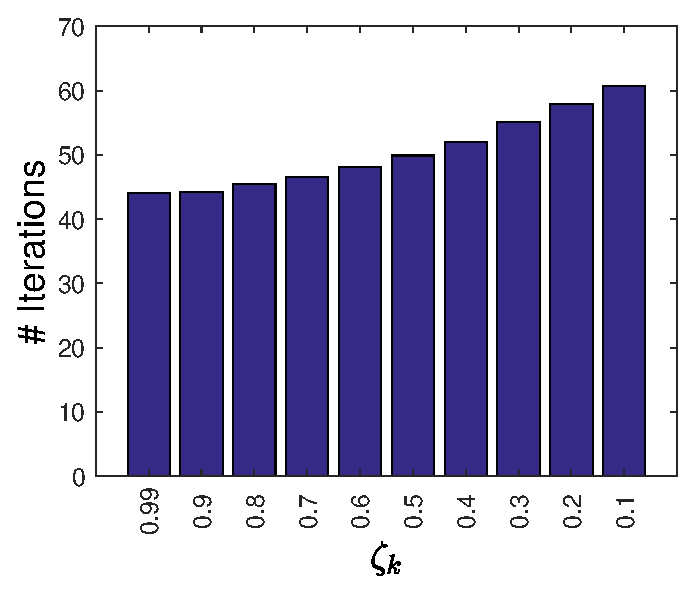
\includegraphics[scale=\myscaleF]{../figures/SDDit} & 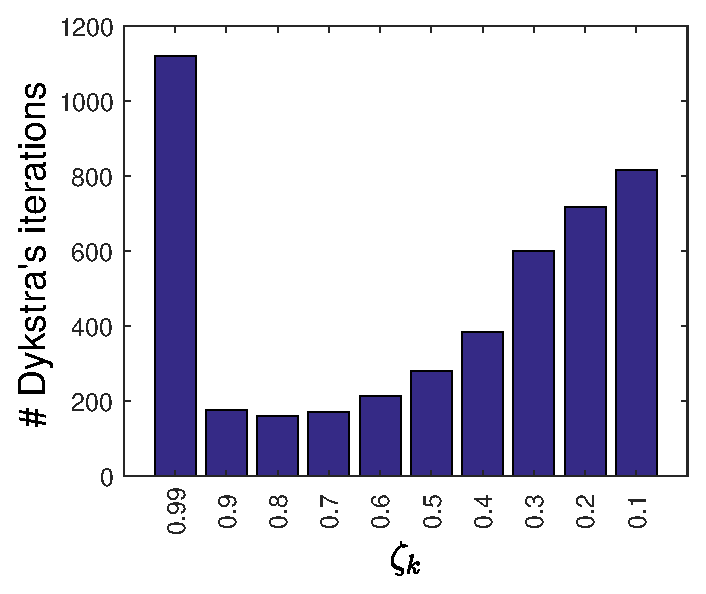
\includegraphics[scale=\myscaleF]{../figures/SDDDIT} & 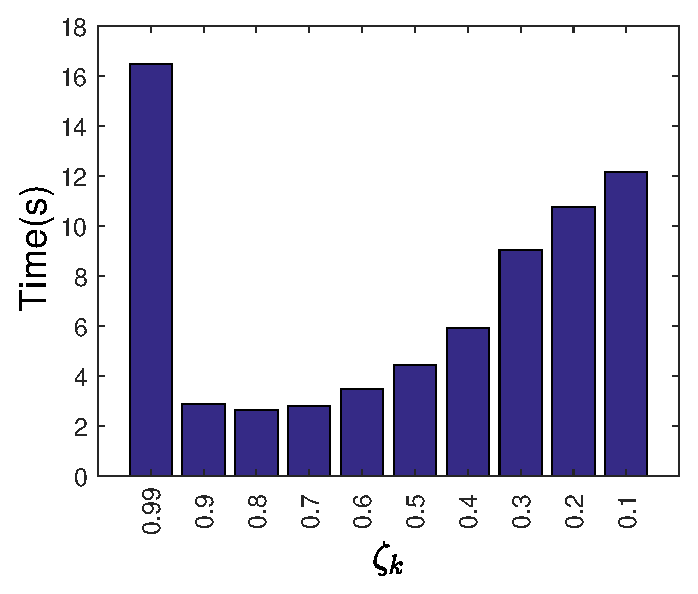
\includegraphics[scale=\myscaleF]{../figures/SDDtime}\\
    (a) & (b) & (c)\\
  \end{tabular}
  \caption{Results for 10 instances of Problem I using $n=100$, $m=200$, and $c=10$. Average number of: (a) iterations; (b) Dykstra’s iterations; (c)  CPU time in seconds needed to reach the solution for different choices of $\zeta_k$.}
\end{figure}   
\end{frame}

\begin{frame}[t]\frametitle{Influence of the inexact projection}    
\begin{figure}[H]\centering
  \begin{tabular}{ccc}
    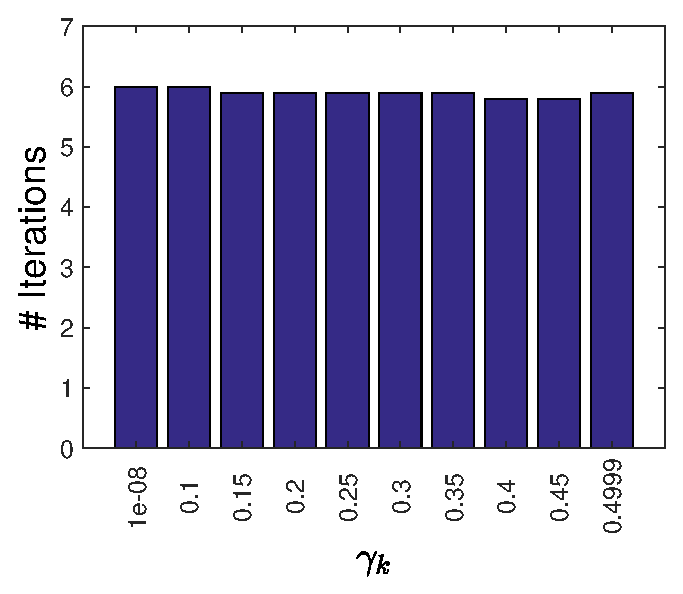
\includegraphics[scale=\myscaleF]{../figures/Specit} & 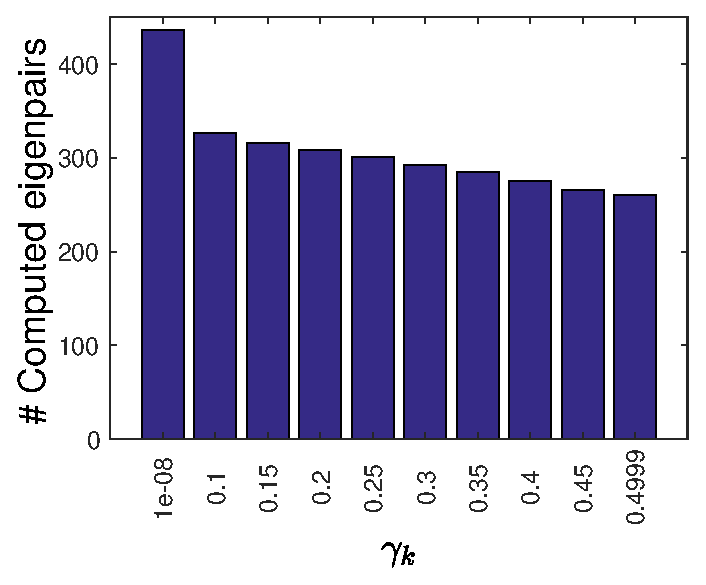
\includegraphics[scale=\myscaleF]{../figures/SpecFWIT} & 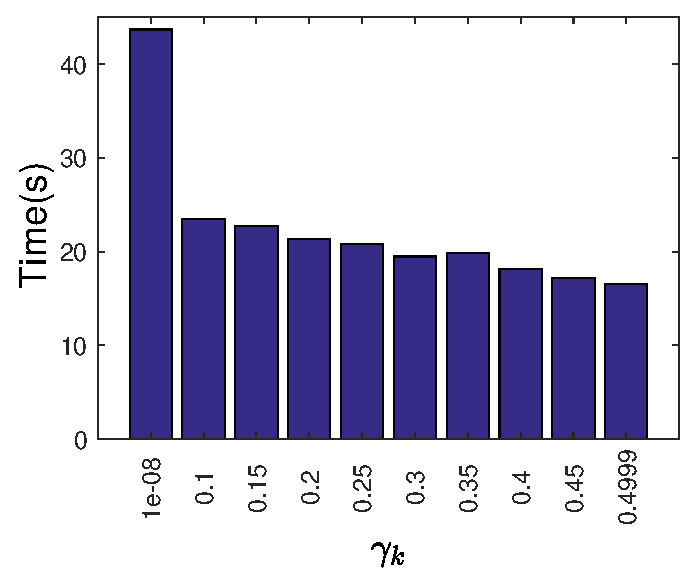
\includegraphics[scale=\myscaleF]{../figures/Spectime} \\
    (a) & (b) & (c)\\
  \end{tabular}
  \caption{Results for 10 instances of Problem II using $n=800$, $m=1000$, and $c=100$. Average number of: (a) iterations; (b) computed eigenpairs; (c)  CPU time in seconds needed to reach the solution for different choices of $\gamma_k$.}
\end{figure}
\end{frame}

\begin{frame}[t]\frametitle{Influence of the line search scheme}
    
\begin{figure}[H]\centering
  \begin{tabular}{cccc}
    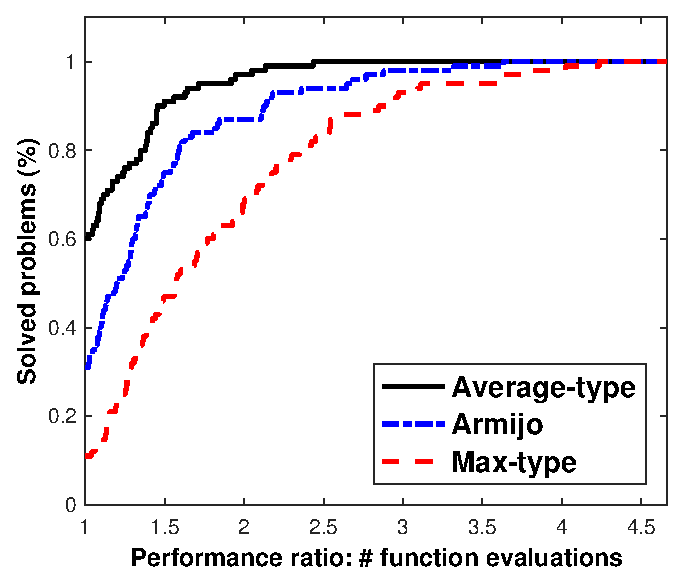
\includegraphics[scale=\myscale]{../figures/ppSDDnfev} &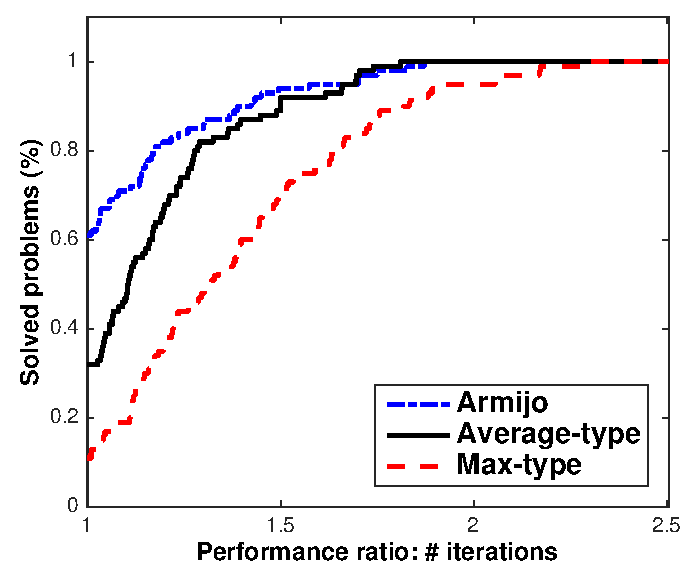
\includegraphics[scale=\myscale]{../figures/ppSDDit} & 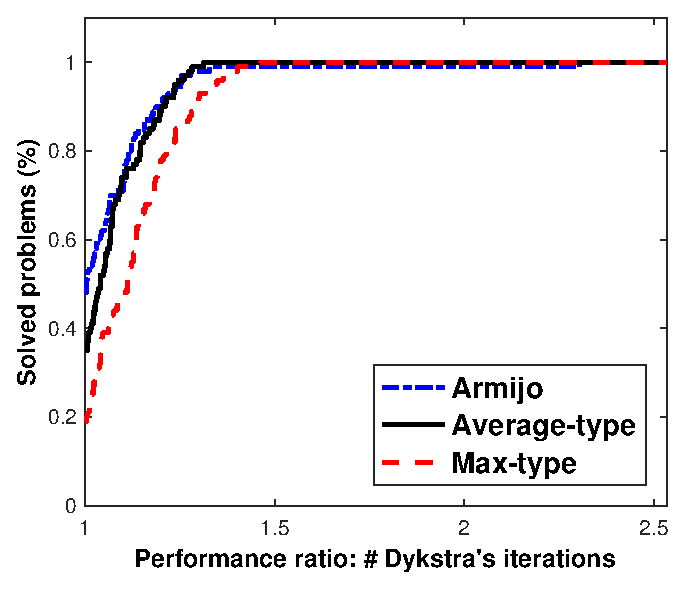
\includegraphics[scale=\myscale]{../figures/ppSDDnDIT} & 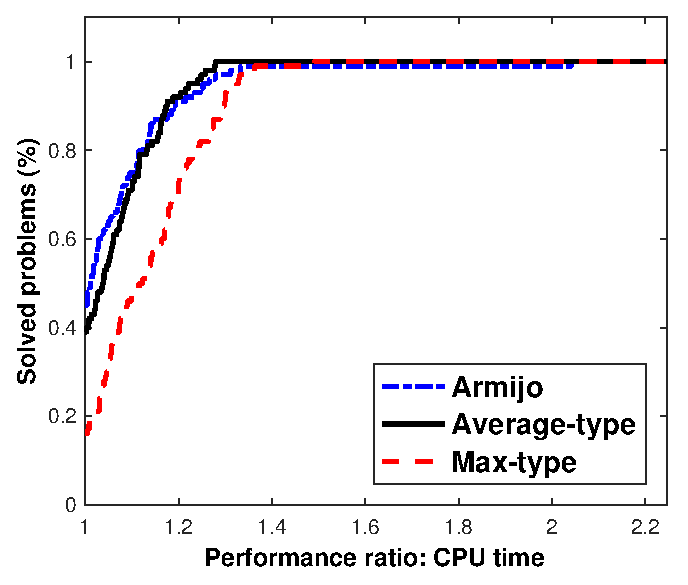
\includegraphics[scale=\myscale]{../figures/ppSDDtime} \\
    (a) & (b) & (c) & (d)\\
  \end{tabular}
  \caption{Performance profiles for Problem~I considering the SPG method with the Armijo, the Average-type, and the Max-type line searches strategies using as performance measurement: (a) number of function evaluations; (b) number of (outer) iterations; (c) number of Dykstra’s iterations; (d) CPU time.}
  
\end{figure}
\end{frame}

\begin{frame}[t]\frametitle{Influence of the line search scheme}
    \begin{figure}[H]\centering
  \begin{tabular}{cccc}
    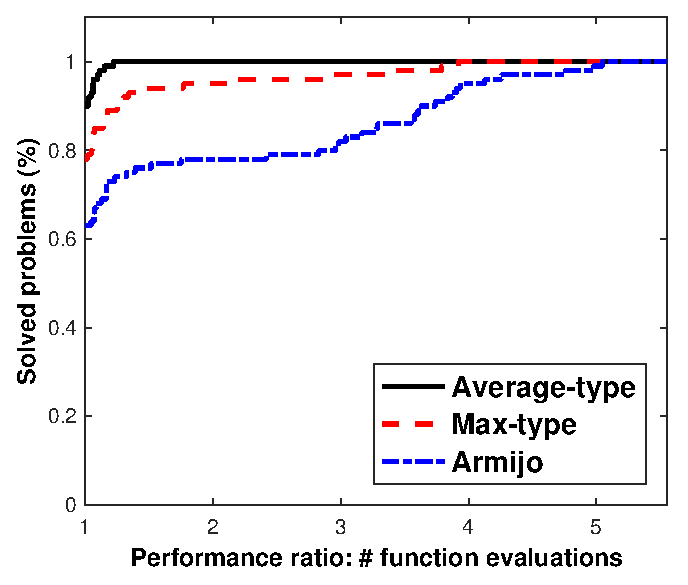
\includegraphics[scale=\myscale]{../figures/ppSpecnfev}&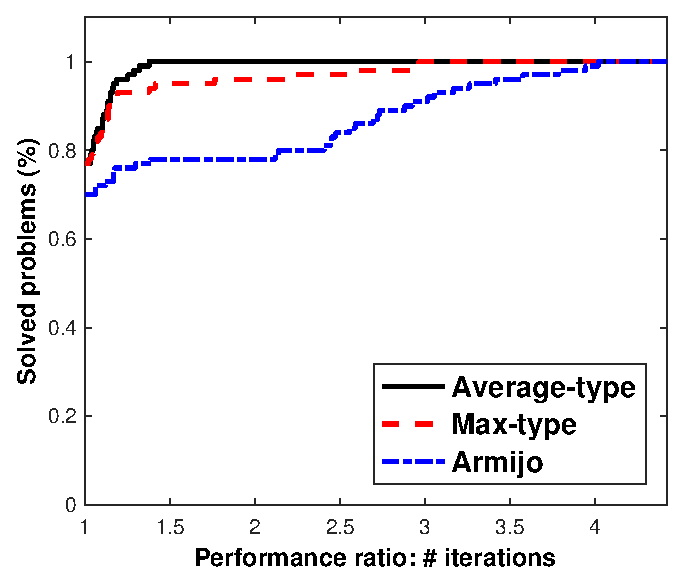
\includegraphics[scale=\myscale]{../figures/ppSpecit} & 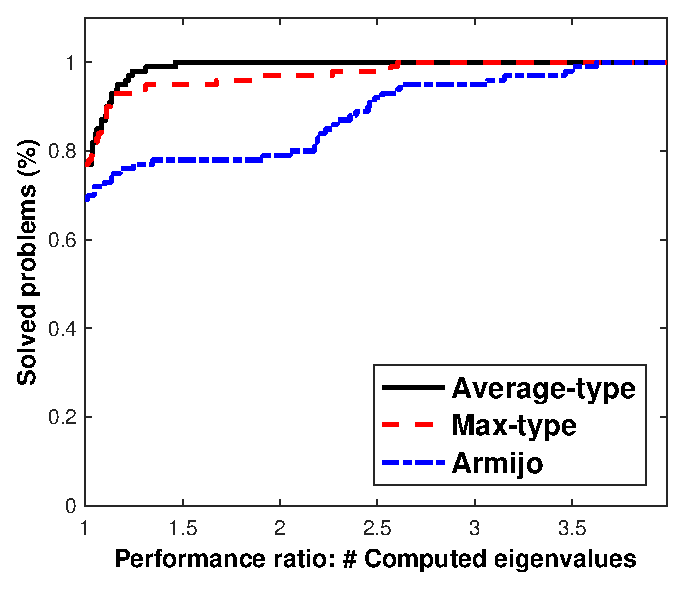
\includegraphics[scale=\myscale]{../figures/ppSpecnFW} & 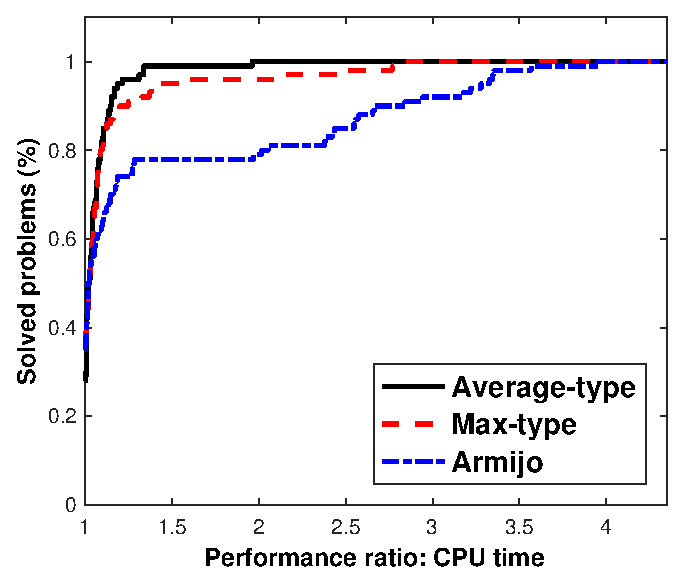
\includegraphics[scale=\myscale]{../figures/ppSpectime} \\
    (a) & (b) & (c) & (d)\\
  \end{tabular}
  \caption{Performance profiles for Problem~II considering the SPG method with the Armijo, the Average-type, and the Max-type line searches strategies using as performance measurement: (a) number of function evaluations; (b) number of (outer) iterations; (c) number of computed eigenpairs; (d) CPU time.}
\end{figure}
\end{frame}
\chapter{Applications} \label{chap:App}

\section{Risks measures}

In this section we discuss different ways to measure the risk of portfolio.


\begin{definition}
	A portfolio with $n$ assets, $A_1, A_2, \dots, A_n$, is a vector $x^\top = (x_1, x_2, \dots, x_n)\in \R^n$ where each coordinate $x_i$ is the weight of capital invested in asset $A_i$.
\end{definition}

Let $L(x,y)$ be the loss associated with the decision vector $x$, to be chosen from a certain subset $X$ of $\R^n$ and the random vector $y \in \R^m$. The vector $x$ can be interpreted as representing a portfolio, with $X$ as the set of available portfolios
(subject to various constraints). The vector $y$ stands for the uncertainties, e.g. in market parameters, that can affect the loss. Of course the loss might be negative and thus, in effect, constitute a gain.

For each $x$, the loss $L(x,y)$ is a random variable having a distribution in $\R$ induced by that of $y$. The underlying probability distribution of $y \in \R^m$ will be assumed to have density, which we denote by $p(y)$.

The probability of $f(x,y)$ not exceeding a threshold $\alpha$ is given then by
\[
	\Psi (x,\alpha) = \int_{L(x,y)\leq \alpha} p(y)\,dy.
\]
As a function of $\alpha$ for fixed $x, \Psi(x, \alpha)$ is the \textit{cumulative distribution function} for the loss associated with $x$. Since $p(y)$ is continuous, $\Psi(x, \alpha)$ is nondecreasing with respect to $\alpha$ and continuous.


The \textit{expected loss} $\mu$ of a portfolio $x$ is given by
\[
	\mu(x) = \int_{\R} L(x,y)\,p(y)\,dy.
\]
Moreover, the \textit{loss variance} of $x$ is
\[
	\sigma^2(x) = \int_{\R} \big(L(x,y)-\mu(x)\big)^2\,p(y)\,dy
\]
and the \textit{volatility} of the loss is $\sigma(x)$.

The volatility of the loss was defined as a \textit{risk measure} to a portfolio by Nobel laureate in economics, Harry Markowitz in 1952 (see in \cite{Markowitz1952}) under the hypothesis of loss has a normal distribution. In the following we see that this choice is not the better one.

In 1999 Artzner, Delbaen, Eber and Heath (see in \cite{Artzner1999}) defined, what they called \textit{coherent risk measure}, from the following axioms to a risk measure $\mathcal{R}$:

\begin{axiom}[Translation invariance] For all portfolio $x$ and all $m\in\mathbb{R}$,  we have
	\[
		\mathcal{R}(x+m) = \mathcal{R}(x)-m.
	\]
\end{axiom}
This means that adding an amount of cash, $m$, to a portfolio decreases your risk by the same amount.

\begin{axiom}[Subadditivity] If $x_A$ and $x_B$ are two portfolios, then
	\[
		\mathcal{R}(x_A+x_B) \leq \mathcal{R}(x_A) + \mathcal{R}(x_B),
	\]
\end{axiom}
In particular, this property means that ``a merger does not create extra risk.''

\begin{axiom}[Positive homogeneity] For all portfolio $x$ and all $\lambda\leq 0$ we have
	\[
		\mathcal{R}(\lambda x) = \lambda \mathcal{R}(x), \qquad \mbox{se } \lambda
		\geq 0.
	\]
\end{axiom}
This property implies that the risk measure is a linear function of the size of the position.

\begin{axiom}[Monotonicity] Let $x_A$, $x_B$ be two portfolios,
	\[
		\mbox{if } x_A \prec x_B, \quad \mbox{then } \quad \mathcal{R}(x_A) \geq \mathcal{R}(x_B).\\
	\]
\end{axiom}
If a portfolio $x_A$ performs worse than $x_B$ in any
scenario $(x_A \prec x_B)$, then it means that the portfolio $x_A$ is
riskier than $x_B$.

\begin{definition}
	A risk measure satisfying the axioms of translation invariance, subadditivity, positive homogeneity, and monotonicity is called \textbf{coherent}.
\end{definition}


When the risk measure is not assumed to have variations proportional to the risk variations themselves, the positive homogeneity is no longer satisfied. Alternative axioms can be proposed.

\begin{axiom}[Convexity] For all portfolios $x_A$, $x_B$ and for all $0\leq \lambda \leq 1$,
	\[
		\mathcal{R}(\lambda x_A + (1-\lambda)x_A) \leq \lambda \mathcal{R}(x_A) + (1-\lambda) \mathcal{R}(x_B).
	\]
\end{axiom}

This axiom  was proposed in 2002 by Föllmer and Shield (see in \cite{Follmer2002}). It means that diversification does not increase risk.

\begin{definition}
	A risk measure satisfying the axioms of translation invariance, monotonicity, and convexity is called \textbf{convex}.
\end{definition}

\begin{proposition}
	A convex risk measure is coherent if it satisfies the positive homogeneity. Note also that the positive homogeneity and the subadditivity implies the convexity.
\end{proposition}

The standard deviation does not satisfy translation invariance, however, this condition was defined with the perspective of banking system risk and is often ignored in case of portfolio construction.

In financial business, some of the risk management requirements are done in terms of loss distribution percentiles. An upper percentile of the loss distribution is called \textit{Value-at-Risk} ($\mbox{VaR}_\beta$)\footnote{By definition, $\mbox{VaR}_\beta$ is the percentile of the loss distribution, i.e., with a specified confidence level $\beta$, the $\mbox{VaR}_\beta$ of a portfolio is the lowest amount $\zeta$ such that, with probability $\beta$, the loss is less or equal to $\zeta$.}. For instance, $\mbox{VaR}_{0.95}$ is an upper estimate of losses which is exceeded with 5\% probability. The popularity of $\mbox{VaR}_\beta$ is mostly related to a simple and easy to understand representation of high losses. $\mbox{VaR}_\beta$ can be quite efficiently estimated and managed when underlying risk factors are normally (log-normally) distributed.

An alternatuve measure of losses is another percentile risk measure which is called \textit{Conditional Value-at-Risk} ($\mbox{CVaR}_\beta$). The $\mbox{CVaR}_\beta$ risk measure is closely related to $\mbox{VaR}_\beta$. For continuous distributions, $\mbox{CVaR}_\beta$ is defined as the conditional expected loss under the condition that it exceeds $\mbox{VaR}_\beta$, see Rockafellar and Uryasev (see \cite{RockafellarUryasev2001}). For continuous distributions, this risk measure also is known as \emph{Expected Shortfall}, \textit{Mean Excess Loss}, \textit{Mean Shortfall}, or \textit{Tail Value-at-Risk}.


\begin{figure}[H]
	\centering
	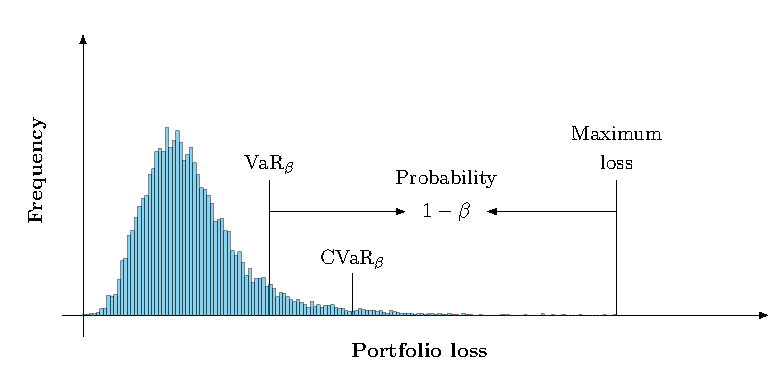
\includegraphics{figures/VarCvar.pdf}
	\caption{Portfolio Loss Distribution, VaR and CVaR}
	\label{fig:VarCvar}
\end{figure}

\begin{remark}\normalfont \hspace{1cm}
	\begin{itemize}
		\item The $\mbox{VaR}_\beta$ answers the question: what is the maximum loss with a specified confidence level $\beta$?
		\item The $\mbox{CVaR}_\beta$ answers the following question: what is the average loss in the $100(1-\beta)$\% worst case scenarios?
	\end{itemize}
\end{remark}

The $\mbox{VaR}_\beta$ and $\mbox{CVaR}_\beta$ values for the loss random variable $L(x,y)$ associated with $x$ and any specified probability level $\beta \in (0,1)$ will be denoted by $\alpha_\beta(x)$ and $\mbox{ES}_\beta(x)$. In our setting they are given by
\begin{equation}\label{eq:var}
	\alpha_\beta(x) = \min\{\alpha\in\mathbb{R} : \Psi(x,\alpha)\geq \beta \},
\end{equation}
and
\begin{equation}\label{eq:cvar}
	\mbox{ES}_\beta(x) = \frac{1}{1-\beta}\int_{L(x,y)\geq \alpha_\beta(x)} L(x,y)\, p(y)\,dy
\end{equation}

Although $\mbox{VaR}_\beta$ is a very popular measure of risk, $\mbox{VaR}_\beta$ is not a coherent risk measure as it does not satisfy subadditivity. 
 














\begin{remark}\normalfont \hspace{1cm}
	\begin{itemize}
		\item The standard deviation does not satisfy condition 4, however, this condition was defined with the perspective of banking system risk and is often ignored in case of portfolio construction.
		\item VaR is not a coherent risk measure as it does not satisfy condition 1. This is a problem because the portfolio’s risk may have be meaningful in this case.
		\item CVaR is a coherent risk measure.
	\end{itemize}
\end{remark}


Let us now assume that the returns are normally distributed, that is, $R\sim N(\mu,\sigma^2)$, where $\mu(x)=x^\top\mu$ and
$\sigma(x)=\sqrt{x^\top \Sigma x}$. Let $\phi(z) = \frac{1}{\sqrt{2\pi}}e^{-z^2/2}$ be the probability density function of Standard Normal Distribution and $\Phi(x) = \int_{-\infty}^{x}\phi(z) dz$
the standard normal accumulated density function.

By definition we have
$P\Big[L(x)\leq \mbox{VaR}_\alpha(x)\Big]=\alpha$, so
$P\Big[R(x)\leq -\mbox{VaR}_\alpha(x)\Big]=1-\alpha$, which standardizing
we have:
\[
	P\left[ \frac{R(x)-x^\top\mu}{\sqrt{x^\top \Sigma x}} \leq \frac{-\mbox{VaR}_\alpha(x)- x^\top\mu}{\sqrt{x^\top \Sigma x}}
		\right]=1-\alpha.
\]
Hence,
\[
	\frac{-\mbox{VaR}_\alpha(x)-x^\top\mu}{\sqrt{x^\top \Sigma x}}=\Phi^{-1}(1-\alpha)
\] and since $\Phi^{-1}(\alpha)=-\Phi^{-1}(1-\alpha)$, we have
\begin{equation}\label{eq:var2}
	\mbox{VaR}_\alpha(x)=-x^\top\mu+ \Phi^{-1}(\alpha)\sqrt{x^\top \Sigma x}.
\end{equation}

This is a special case of the standard deviation-based risk measure with $c = \Phi^{-1} (\alpha)$. It implies that the value-at-risk is a coherent and convex risk measure if the asset returns are normally distributed. The expression of the expected shortfall is:

\[
	\mbox{ES}_\alpha(x) = \frac{1}{1-\alpha}\int_{\mbox{VaR}_\alpha(x)}^\infty u p(u)du,
\] considering $p(u)$ the normal density function, we have that:
\[
	\mbox{ES}_\alpha(x) = \frac{1}{1-\alpha}\int_{-\mu(x)+ \sigma(x)\Phi^{-1}(\alpha)} ^\infty \frac{u}{\sigma(x)\sqrt{2\pi}} e^{-\frac{1}{2}\Big(\frac{u+\mu(x)}{\sigma (x)}\Big)^2} du,
\]

With the variable change
$t=\frac{u+\sigma(x)}{\sigma(x)}$, we obtain

\[
	\begin{aligned}
		\mbox{ES}_\alpha(x) & = \frac{1}{1-\alpha}\int_{\Phi^{-1}(\alpha)}^\infty (-\mu(x)+ \sigma(x)t) \frac{1}{\sqrt{2\pi}} e^{-t^2/2}dt \\
		                    & = -\frac{\mu(x)}{1-\alpha}[\Phi(t)]_{\Phi^{-1}(\alpha)}^\infty +
		\frac{\sigma(x)}{(1-\alpha)\sqrt{2\pi}}\int_{\Phi^{-1}(\alpha)}^\infty t e^{-t^2/ 2}dt                                             \\
		                    & =-\mu(x) + \frac{\sigma(x)}{(1-\alpha)\sqrt{2\pi}}\Big[-e^{-t^2/2} \Big] _{\Phi^{-1}(\alpha)}^\infty         \\
		                    & = -\mu(x) + \frac{\sigma(x)}{(1-\alpha)\sqrt{2\pi}}e^{-\frac{[\Phi^{-1}(\ alpha)]^2}{2}}
	\end{aligned}.
\]

So CVaR can be calculated by
\begin{equation}\label{eq:cvar2}
	\mbox{ES}_\alpha(x)=-x^\top \mu + \frac{\phi(\Phi^{-1}(\alpha))}{1-\alpha}\sqrt{x^ \top \Sigma x}.
\end{equation}
Like the value-at-risk, it is a standard deviation-based risk measure with $c ={\phi(\Phi^{-1}(\alpha))}/{(1-\alpha)}$
In the Gaussian world, different risk measures can be calculated using the expected return and volatility. Note by (\ref{eq:var2}) and (\ref{eq:cvar2}), that both Var and CVaR are the form $-\mu(x)+c\sigma(x)$. In general, we want a portfolio with positive returns, that is, $\mu(x)\geq0$. If the portfolio manager has very optimistic forecasts, component $\mu(x)$ may substantially reduce the risk measure. This explains why omitting the mean component is standard practice in the asset management industry.

\begin{example}\normalfont
	We consider three stocks $A$, $B$ and $C$ whose current prices are respectively $\$ 15.00$, $\$ 25.00$ and $\$ 30.00$. We assume that their expected returns are equal to $30$ bps\footnote{1 bps or one basis point is equivalent to
		0.01\% (the hundredth part of 1\%) or 0.0001 in decimal form.}, $50$ bps and $20$ bps on a daily basis and their daily volatilities are $3\%$, $2\%$, and $1\%$ respectively. The asset correlation matrix is given by
	\[
		\rho = \left(
		\begin{array}{rrr}
				1.00 & 0.40 & 0.15 \\
				0.40 & 1.00 & 0.60 \\
				0.15 & 0.60 & 1.00
			\end{array}
		\right)
	\]

	We consider a portfolio composed by $100$ stocks $A$, $200$ stocks $B$ and $100$ stocks $C$. The value of this portfolio is $\$ 9,500.00$, being $\$ 1,500.00$ invested in stock $A$, $\$ 5,000.00$ in stock $B$ and $\$ 3,000.00$ in stock $C$, therefore the weights of the stocks in this portfolio are $15.79\%$, $52.63\%$, and $31.58\%$ respectively, so $x=(0.1579;\;0.5263;\; 0.3158)$. The expected return on the portfolio is $\mu(x) = 30\times0.1579+50\times0.5263+20\times0.3158$, that is, $\mu(x) = 37$ bps. Using the relationship $\Sigma_{i,j}=\rho_{i,j}\sigma_1\sigma_j$ we find the covariance matrix
	\[
		\Sigma = \left(
		\begin{array}{llr}
				9.0 & 2.4 & 4.5 \\
				2.4 & 4.0 & 1.2 \\
				4.5 & 1.2 & 1.0
			\end{array}
		\right)\times10^{-4},
	\] since the volatility of portfolio is given by $\sigma^2(x) = x^\top \Sigma x$, we have that $\sigma(x) = 1.51\%$.

	Considering $\alpha = 0.99$, we have $\Phi^{-1}(0.99) = 2.325$ and
	$\phi(\Phi^{-1}(0.99))=\phi(2.325)=2.68\%$. Using the equations
	$(\ref{eq:var2})$ and $(\ref{eq:cvar2})$ we have

	\[
		\begin{aligned}
			\mathrm{VaR}_{99\%}(x) & = -0.37\% + 2.325 \times 1.51\% = 3.14\%              \\
			\mathrm{ES}_{99\%}(x)  & = -0.37\% + \frac{2.68}{0.01} \times 1.51\% = 3.68\%.
		\end{aligned}
	\]

	Risk can also be expressed in monetary terms, in this case,

	\[
		\begin{aligned}
			\mathrm{VaR}_{99\%}(x) & = 3.14\% \times \$ 9,500.00 = \$ 298.30  \\
			\mathrm{ES}_{99\%}(x)  & = 3.68\% \times \$ 9,500.00 = \$ 349.60.
		\end{aligned}
	\]
	According to the result of {\rm VaR}, in $99\%$ of the days, the loss will be less than $\$ 298.30$, however in the $1\%$ of the remaining days the {\rm VaR} does not measure how much great can be the loss, this is the role of {\rm CVaR} which indicates that the average loss will be $\$ 349.60$ on the worst $1\%$ days.
\end{example}





\section{The Gaussian Case}

\section{Case Study}




%           References      --------------------------------------
\topskip=2cm\advance\textheight by -2cm\enlargethispage{-1cm}

% \nocite{} % incluir sem citar no texto
% \nocite{*} % Citar todos

\printbibliography
%-----------------------------------------------------------------

\begin{frame}[c]\frametitle{}
	\centering
	\Huge \textbf{Thank you!}
\end{frame}
%-----------------------------------------------------------------
\end{document}
%-----------------------------------------------------------------